\documentclass[lang=cn,12pt,newtx]{elegantbook}

\title{西浦博士生非官方攻略}
\subtitle{~~~~~~~~~~~~~~~~~~~~~~~~~~~~~~~~~~~~版本 v0.4.4}
% \subtitle{111}

\author{热心同学们}
% \institute{}
\date{\today}
% \version{0.3.3}
\bioinfo{不定时更新,最新版下载地址}{\href{https://github.com/kaiwu-astro/xp_pgrs_unofficial_guide/releases}{点击链接}}
% \bioinfo{自定义}{信息}

\extrainfo{前人栽树,后人乘凉~~\&~~吃水不忘挖井人} 

\setcounter{tocdepth}{3}

% \logo{logo-blue.png} 
\cover{cover2.jpg}

% 本文档命令
\usepackage{array}
\usepackage{float}
\usepackage{ulem}
\usepackage{xurl}
\usepackage[export]{adjustbox}
\usepackage{subcaption}
\usepackage{xcolor}
\usepackage{tcolorbox}

\newcommand{\ccr}[1]{\makecell{{\color{#1}\rule{1cm}{1cm}}}}
\newcommand{\emptyline}{\vspace{5mm}}
\newenvironment{newminipage}[1][0.55]
    {   \setlength{\parindent}{0\ccwd}
        \begin{minipage}{#1\textwidth}
            \setlength{\parindent}{2\ccwd}
    }
    {   \end{minipage}
        \setlength{\parindent}{2\ccwd}
    }

% 修改标题页的橙色带
\definecolor{customcolor}{RGB}{3,31,115}
\colorlet{coverlinecolor}{customcolor}
\usepackage{cprotect}

\begin{document}

\maketitle
\frontmatter


\chapter{前言}
\thispagestyle{empty}
{\kaishu{我之前跟一些博士、硕士生同学交流的时候,他们有的都快毕业了,有的都不知道可以去领办公用品,还有的甚至学校体育馆在哪里都不清楚,更别说免费的健身房、球场资源。以及在博士生微信群里,每年都有人到了第一次APR的时间才知道还有meeting record需要填。再以及,利物浦账号下的大量数字资源,了解的人就更少了。有些重要的事,自己不知道,导师不知道,办公室同学也不知道,那最后真的就可能等到毕业了才知道。

这就是发起本攻略项目的目的。虽然说每个同学入学的时候都收到了一本学校发的PGRS Handbook,但很遗憾的是,远远不够。一来其中缺少很多内容,例如利物浦meeting record、利物浦账户福利几乎没介绍;二来由于是全英文,翻了几页干货又不多,估计很多同学像我一样直接就失去了阅读兴趣;三来入学时发了一大堆材料,虽然官方手册有其重要性,但很容易就淹没在那一堆材料里了。

因此我就想到可以克服原手册的弊端,把这些经验记录下来,以泽后人。与我而言,也是作为一名党员为西浦集体做出的微小贡献。也希望受益于本手册同学,能在学习中把自己宝贵的经验记录下来,将帮助传递下去。

本手册并不想替代PGRS Handbook,而只是作为补充以及重点摘录。因此希望看到这本书的同学,有空的时候还是把官方手册从杂物堆里捡起来,很可能有重要的发现。

\begin{flushright}
吴开\\
2022年8月18日于MB
\end{flushright}

\begin{center}
    \begin{large}
        \color{red}{v0.1 note: 目前后面目录里的所有子节都是我随便想的idea,可加可删。
        
        欢迎大家直接投稿填充这些idea,也欢迎自己加。
        
        如何投稿见最后一章(\hyperref[chapter.author-ins]{链接}) }
    \end{large}
\end{center}

}}

\tableofcontents
\mainmatter
%======================================================================
% 正文内容
% \pagestyle{fancy}
% \setcounter{page}{0}
%# -*- coding: utf-8-unix -*-
%%==================================================
\chapter{Start here: 入口级网站和应用}
\label{necessary_resources}

\begin{flushright}
    ——据说99\%的博士生都收藏了这些
\end{flushright}    

\section{网站}
\begin{itemize}
    \item 西浦校内网站导航:\url{https://guide.xjtlu.edu.cn}
    \item 个人信息门户ebridge:\url{https://ebridge.xjtlu.edu.cn}
    \item 利物浦信息门户Liverpool Life:\url{https://liverpool-life.liverpool.ac.uk}
\end{itemize}

\section{公众号}

\begin{table}[H]
    \begin{tabular}{ccc}
        \begin{subfigure}{0.25\columnwidth}
            
\includegraphics[width=\linewidth]{author-folder/Kai.Wu/qrcode_XJTLU-China_1.jpg} \caption{学校公众号}
        \end{subfigure} \hfill
        \begin{subfigure}{0.25\columnwidth}
            
\includegraphics[width=\linewidth]{author-folder/Kai.Wu/qrcode_XJTLU_library_1.jpg} \caption{图书馆}
        \end{subfigure} \hfill
        \begin{subfigure}{0.25\columnwidth}
            
\includegraphics[width=\linewidth]{author-folder/Kai.Wu/qrcode_student_service.jpg} \caption{学生服务(一站式)}
        \end{subfigure} \hfill
        \begin{subfigure}{0.25\columnwidth}
            
\includegraphics[width=\linewidth]{author-folder/Kai.Wu/qrcode_IT.jpg} \caption{IT}
        \end{subfigure} \hfill
    \end{tabular}
\end{table}

另外,各学院可能有公众号,可在微信搜 “西浦\ {学院名}" "西交利物浦\ {学院名}"

\section{手机APP}
\url{https://guide.xjtlu.edu.cn/How-to-install-the-XJTLU-APP.html}

\section{常用资源位置}
\begin{itemize}
    \item 西浦PGR Handbook电子版、学校政策、校规:登录ebridge,在中间的PGR Policies, Procedures and Forms里
    \item 利物浦PGR Handbook电子版 \url{https://www.liverpool.ac.uk/student-administration/research-students/pgr-handbook/}
    \item 校园地图:见附录 Chapter.\ref{sec.appendix}。或者微信搜“西浦地图”小程序
    \item 校历:见附录 Chapter.\ref{sec.appendix}
    \item 常用电话:见附录 Chapter.\ref{sec.appendix}
\end{itemize}


%# -*- coding: utf-8-unix -*-
%%==================================================
\chapter{这些必须得做,不然毕不了业}
\label{must-do}

\section{必修课程}
学校为博士生提供了一系列的课程,会在learning mall的页面公布(\href{https://core.xjtlu.edu.cn/course/view.php?id=847}{链接在此}),也会以\textit{Updates on Workshops for Postgraduate Research Students}为题的邮件通知大家。绝大部分的课程大家依照自己的水平选择参加,但是,其中有两门是必须要参加的,否则没法毕业。分别是

\begin{itemize}
    \item Supervisor-Supervisee Relationships
    \item Research Integrity (Ethics)
\end{itemize}

这两个workshop,每个\textbf{学期}都有,但在毕业之前务必参加分别一次,以参加时扫码签到情况为准。

\begin{flushright}
(2022年10月07日 by Kai Wu)
\end{flushright}

\section{Liverpool Life 会议记录}
\label{sec.meeting_record}
作为APR要求的一部分,每位同学作为利物浦的博士生,必须要在一个称作Liverpool-life的系统里,记录自己和导师的会议时间和内容。下面为大家演示一下如何操作。

\begin{enumerate}
    \item 首先进入liverpool-life网站\url{https://liverpool-life.liverpool.ac.uk/},用你的利物浦学号(不是邮箱,更不是西浦学号)和密码登录
    \item 点击左侧的PGR Toolbox
    \begin{figure}[H]
        \centering
        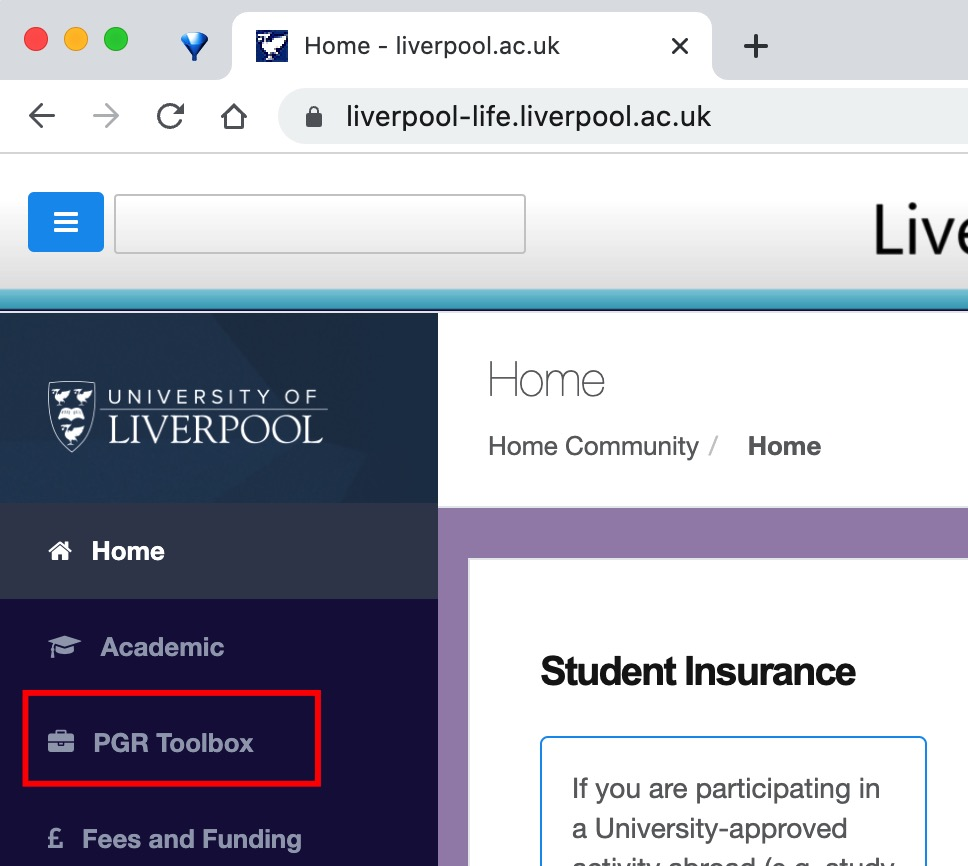
\includegraphics[width=0.5\columnwidth]{author-folder/Kai.Wu/meeting_record_figures/toolbox.jpg}
    \end{figure}
    \item 往下拉,找到PGR Record of Supervisory Meetings,点击View all meetings
    \item 点击Arange new meeting,会弹出窗口,填入日期时间,选择导师(在你后面全部填写完过后,被选中的导师会在他的利物浦邮箱收到邮件)。取消勾选第一个create calendar appointment,否则会在利物浦邮箱的日历里创建一个多半用不上的日程(因为西浦的学生一般都用西浦邮箱对应的日历系统,利物浦的日历系统应该是从来不用的),然后勾选下面的has been pre-agreed。
    \begin{figure}[H]
        \centering
        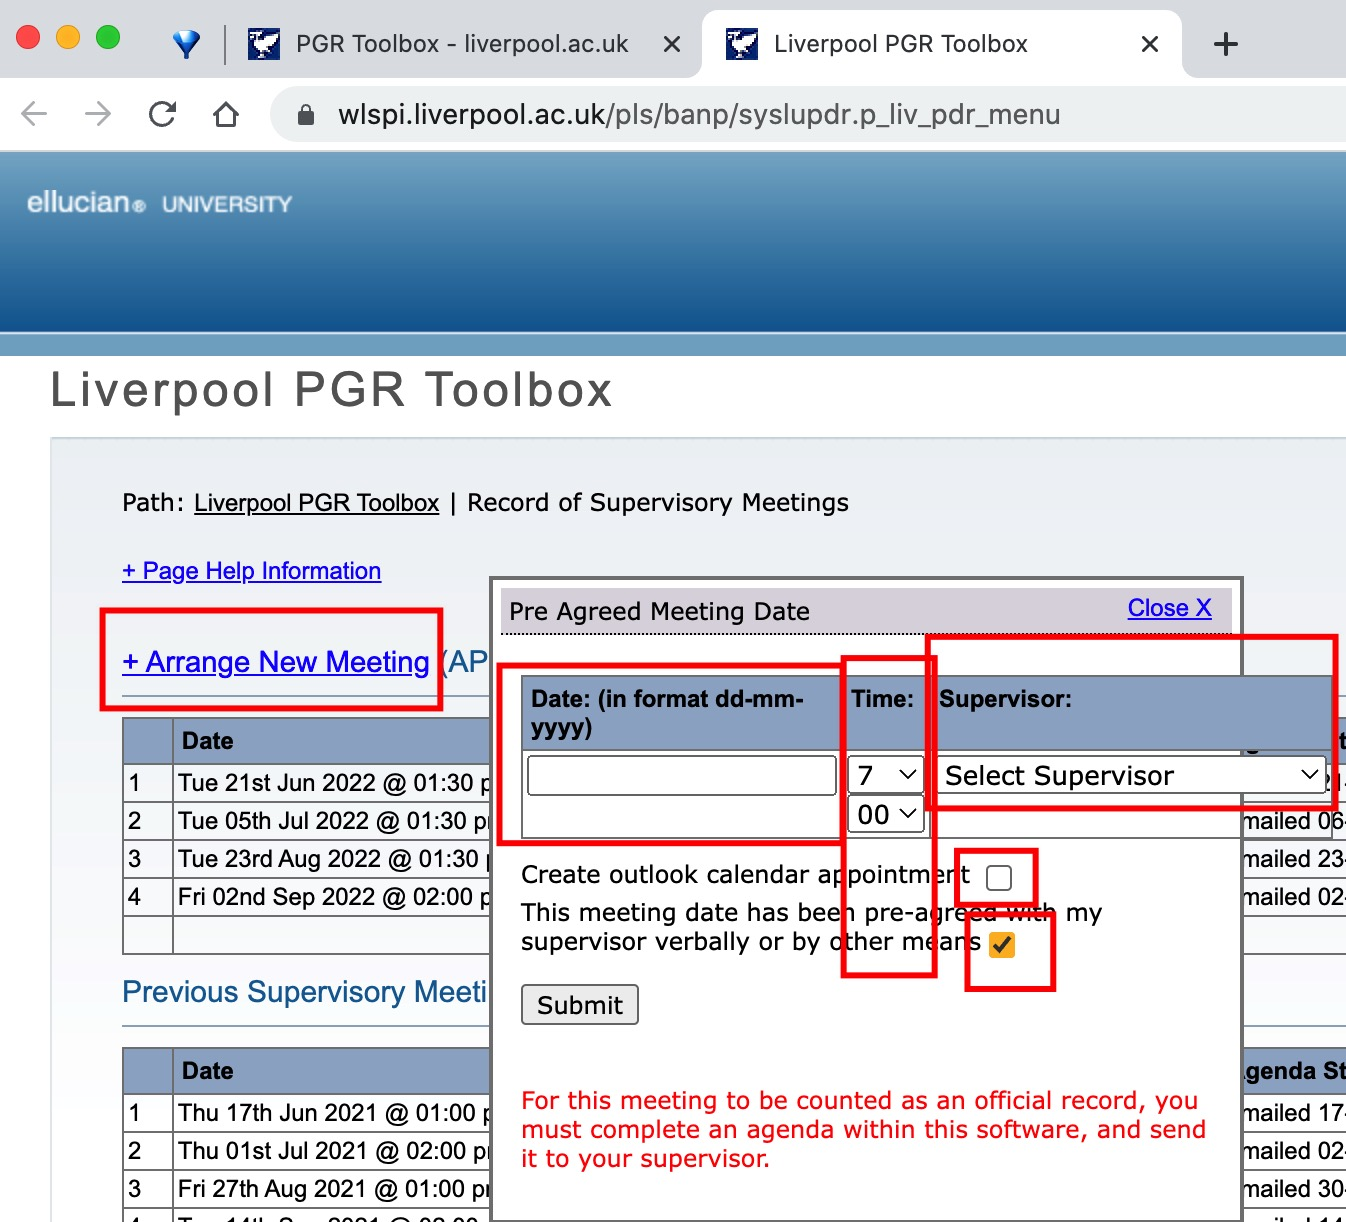
\includegraphics[width=0.5\columnwidth]{author-folder/Kai.Wu/meeting_record_figures/arange_new_meeting.jpg}
    \end{figure}
    \item 然后回忆一下你最近一次跟导师meeting时谈论的内容,填写进度报告(你做了什么)、target(直到下次meeting前打算做什么)、讨论项目
    \begin{figure}[H]
        \centering
        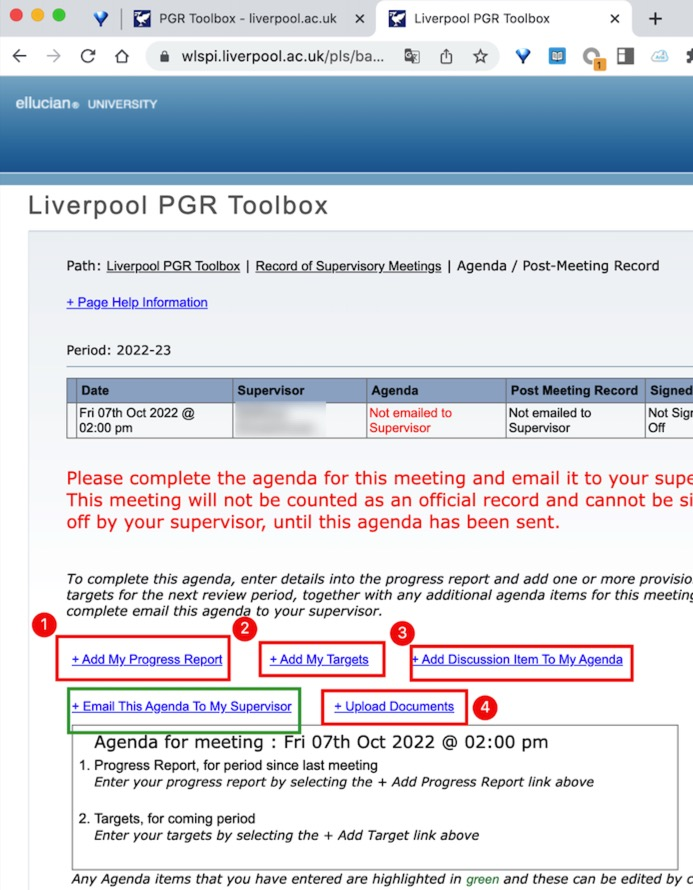
\includegraphics[width=0.5\columnwidth]{author-folder/Kai.Wu/meeting_record_figures/add_items_to_meetings.jpg}
    \end{figure}
    \item 内容不用太多,但也不能太敷衍,毕竟利物浦是要检查的。填完过后,点击email this agenda,然后你和你导师的利物浦邮箱都会收到一封系统自动生成的邮件。
    \begin{figure}[H]
        \centering
        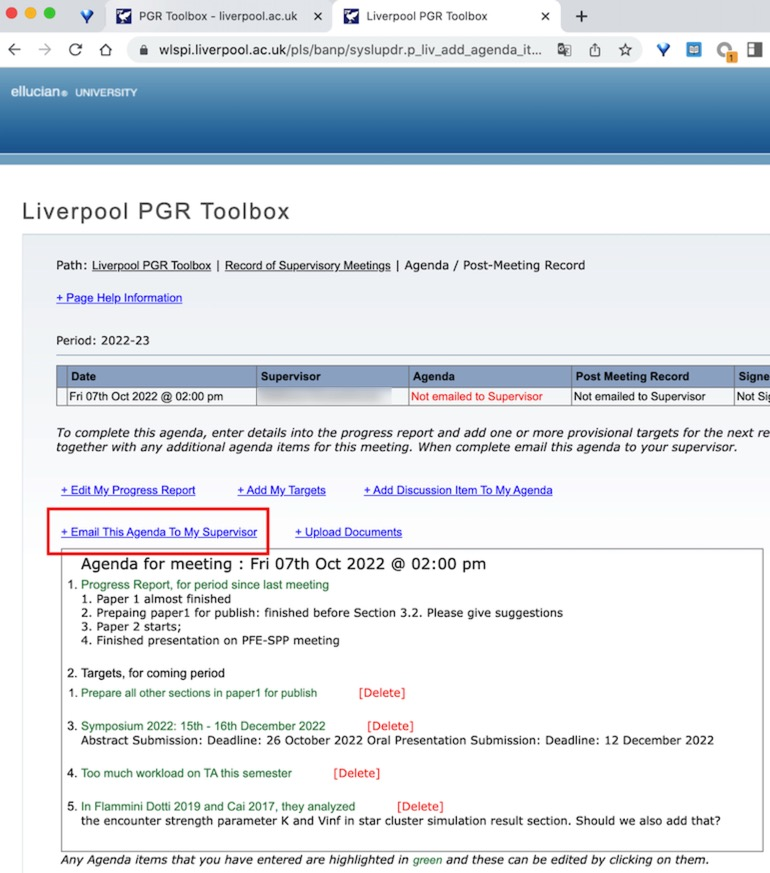
\includegraphics[width=0.5\columnwidth]{author-folder/Kai.Wu/meeting_record_figures/email_to.jpg}
    \end{figure}
    \item 到这里不要着急关闭,还要填一下你们会议中的意见。点击右边的view edit meeting
    \begin{figure}[H]
        \centering
        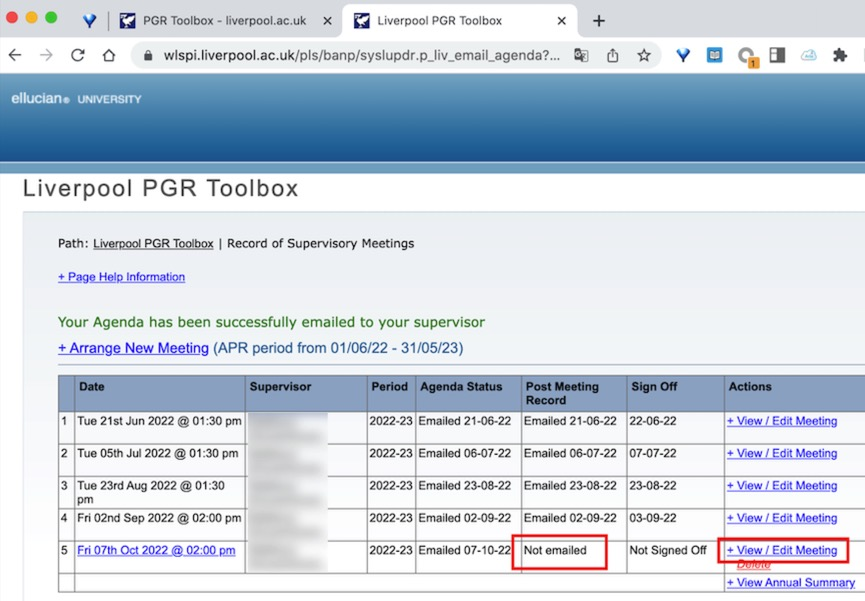
\includegraphics[width=0.5\columnwidth]{author-folder/Kai.Wu/meeting_record_figures/view_edit.jpg}
    \end{figure}
    \item 填入会议中的意见。最后点左上角email,你和导师的利物浦邮箱又会收到一封邮件
    \begin{figure}[H]
        \centering
        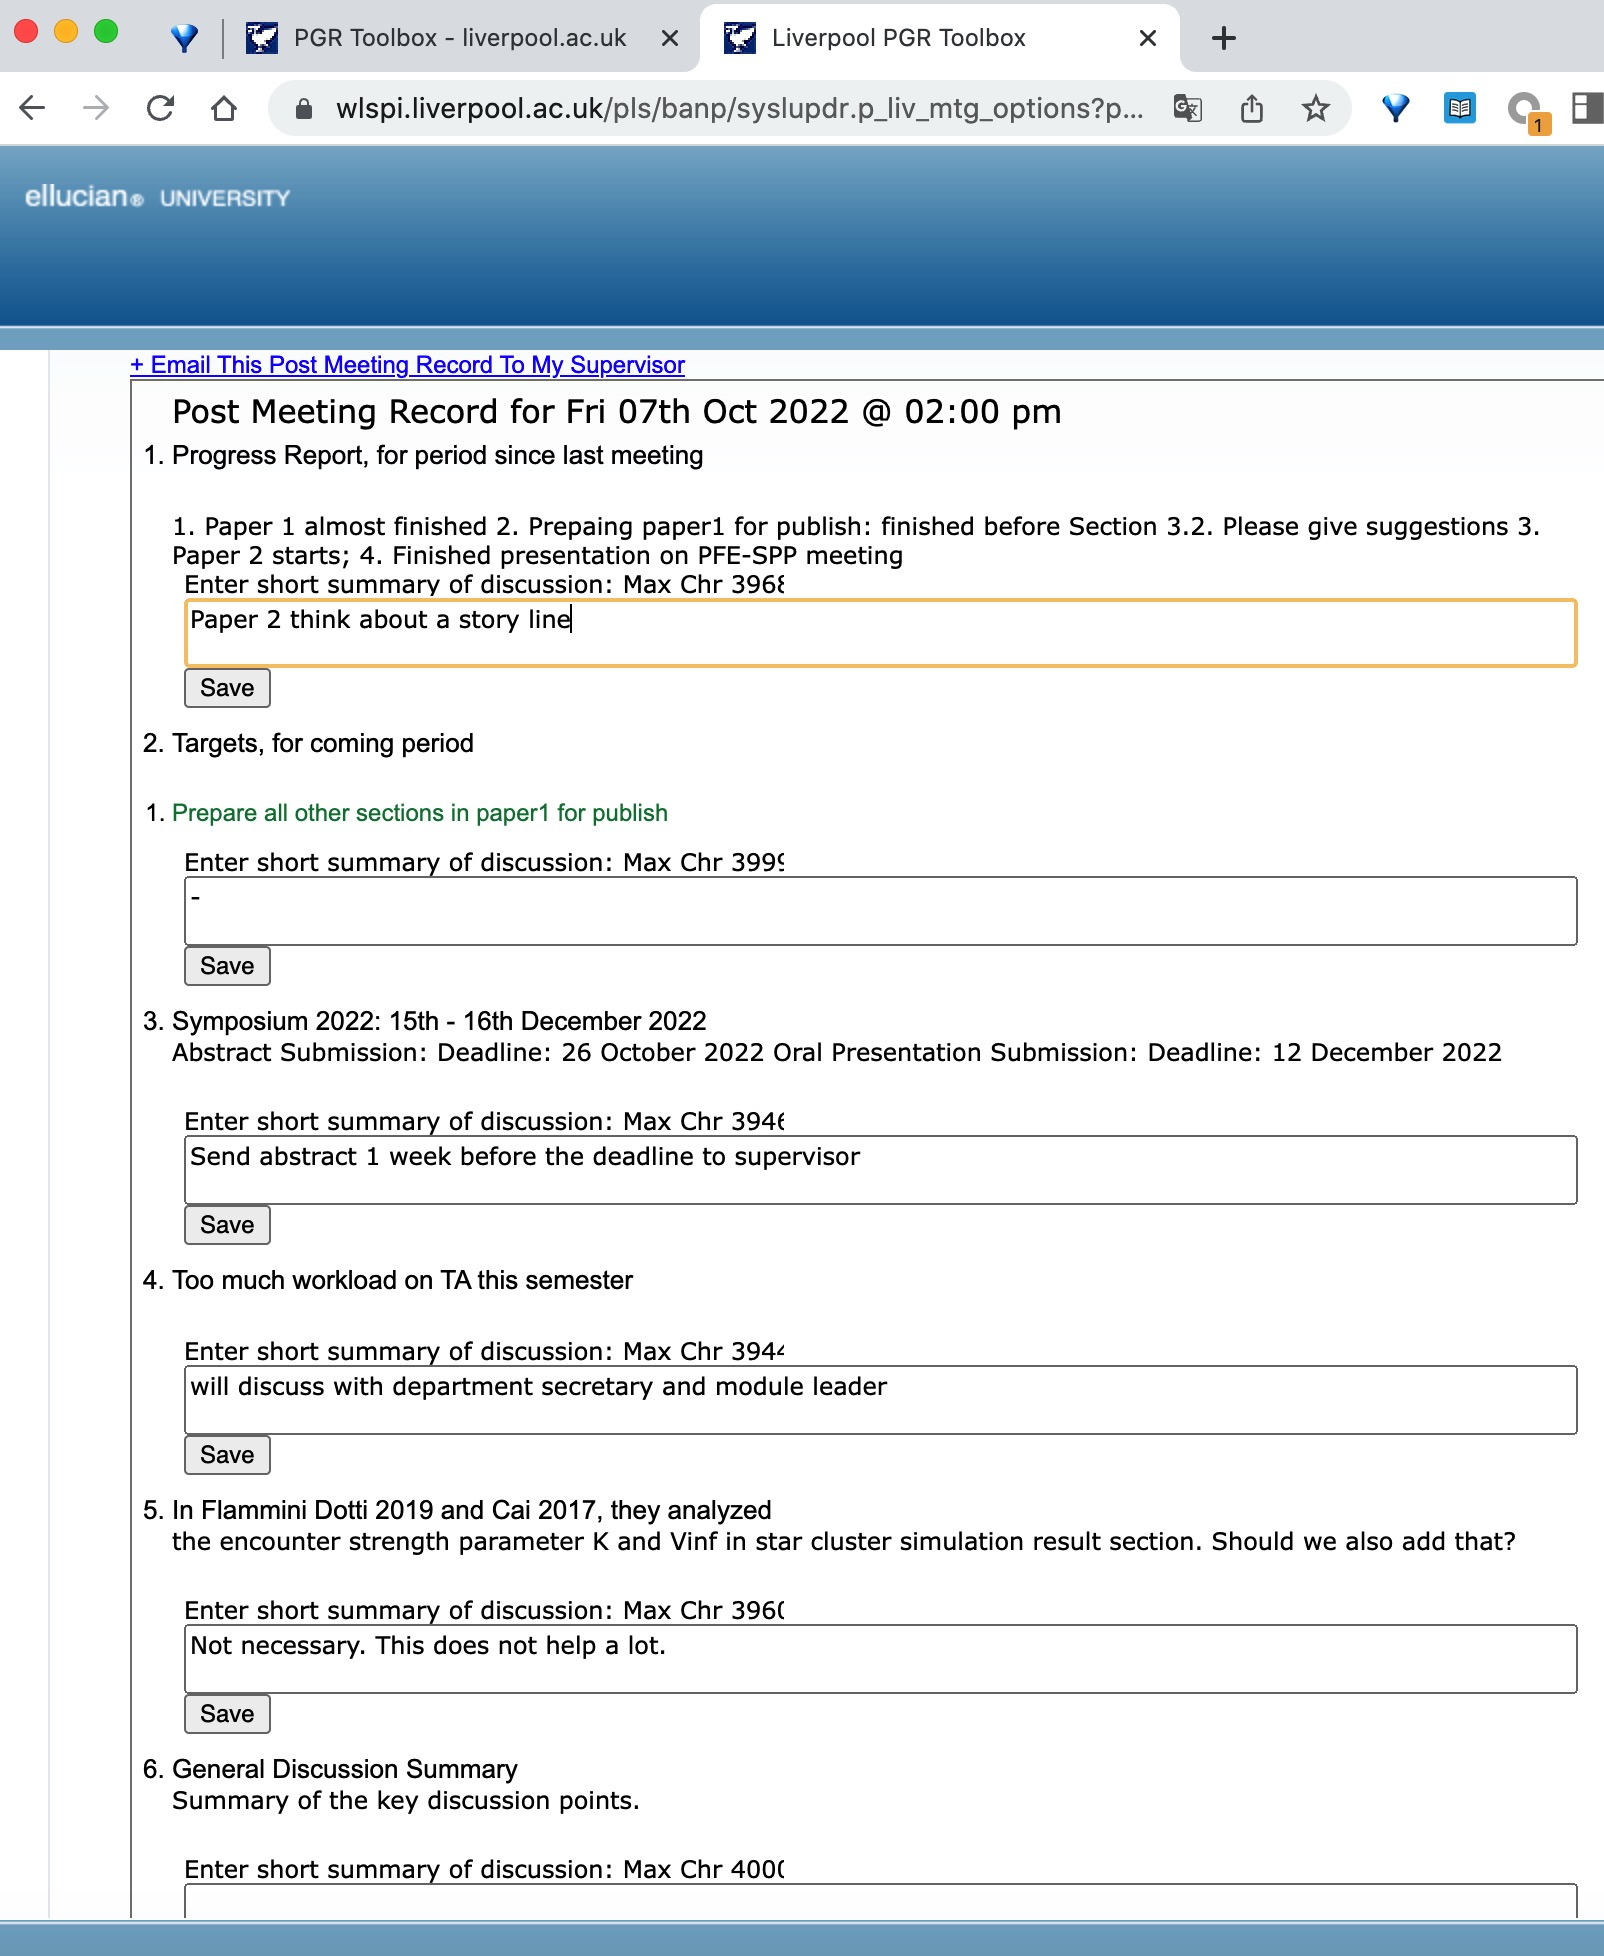
\includegraphics[width=0.5\columnwidth]{author-folder/Kai.Wu/meeting_record_figures/post_meeting.jpg}
    \end{figure}
    \item 
        \begin{minipage}{0.3\textwidth}
            由于liverpool life的尿性,建议最后在liverpool life的界面,点击右上角手动登出,否则下次可能很难登录进去
        \end{minipage}
        \begin{minipage}{0.7\textwidth}
            \begin{figure}[H]
                \centering
                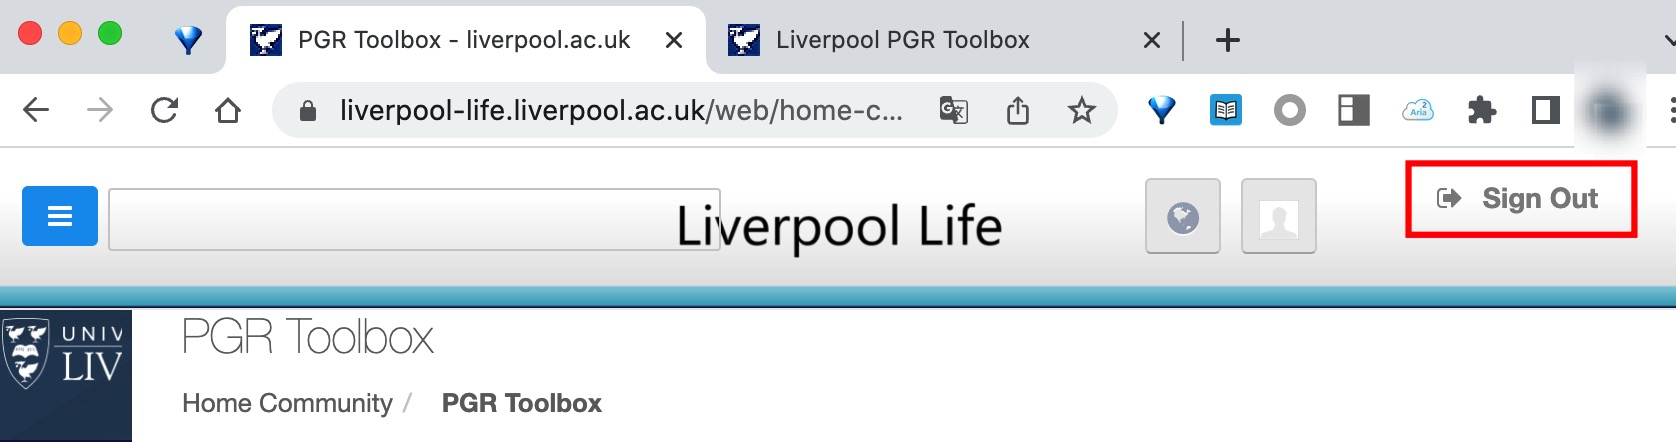
\includegraphics[width=0.9\columnwidth]{author-folder/Kai.Wu/meeting_record_figures/sign_out.jpg}
            \end{figure}
        \end{minipage}
    % \begin{figure}[H]
    %     \centering
    %     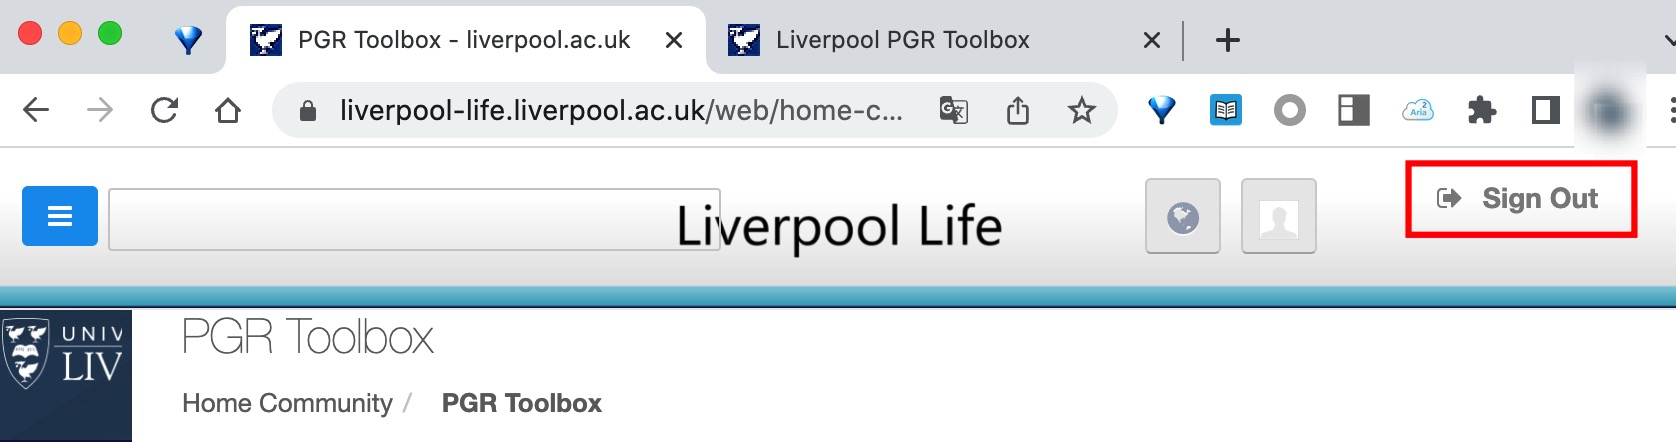
\includegraphics[width=0.5\columnwidth]{author-folder/Kai.Wu/meeting_record_figures/sign_out.jpg}
    % \end{figure}
    \item 到这里你要做的就结束了。你导师需要在他利物浦邮箱收到的邮件里,点击sign off,之后你的利物浦邮箱会收到一封题为 \textit{PGR Supervisor Meeting 5 (Fri 07th Oct 2022 @ 02:00 pm): sign off comments} 的邮件,然后这次meeting record才算全部完成。每年APR之前,必须要每月至少1次的meeting全部sign off。如果你的导师一直没sign off,需要提醒他
\end{enumerate}

\vspace{5mm}
【几个注意事项】
\begin{itemize}
    \item 这个记录最好是每个月填一次。虽然可以补,就是几个月不填然后一口气补半年的,这样是被允许的,但是不规范。我个人的经验里,如果放到APR前夕来补,一来也忘了当年的进度到底是什么,二来APR前夕也很忙。所以,尽量还是按要求每月填一次吧
    \item liverpool life和这个填报网站,经!常!登!不!上!去!因为各种网络和系统的问题,反正即使在西浦校内用wifi和网线都是概率登得上去。据各位同学亲测,一般自己使用科学上网,开全局代理,连通性会好很多,但这些不太合法的方法不能教给大家,也万万不能在微信、QQ里讨论,否则会封号、炸群。不会科学上网的同学,更是要尽量早填报,否则到deadline登不上去就更着急。
\end{itemize}

\begin{flushright}
    (2022年10月10日 by Kai Wu)
    \end{flushright} \clearpage

\section{APR}
\subsection{APR 是什么}
首先请看官方说明。没看过的同学,请务必逐字逐句阅读完毕,因为APR重要性相当于一次小答辩 

\url{https://www.liverpool.ac.uk/student-administration/research-students/progression/annual-progress/}

在我的理解里,APR的作用是
\begin{itemize}
    \item Interview: 读PhD本身很不容易,所以学校、学院需要了解学生遇到的问题,帮助解决
    \item Seminar: 锻炼作报告的能力 + 认识其他博士生同学
    \item Progress report: 了解学生进度,进一步发现并帮助解决学生遇到的问题。同时,筛查完全不认真学习的学生
\end{itemize}

有同学一开始面对APR的时候会很紧张,因为如果APR不通过,直接会被退学。但实际上APR主要是帮助大家解决问题的,只要你不是确实主观上不愿意读,一年以来几乎没做事情,一般都不会不通过。所以,反而应该大胆的在APR里暴露自己的问题,寻求帮助。

\subsection{APR 流程}
\subsubsection{准备工作}
APR的前置任务只有一个,那就是要填完\textbf{每月至少一次}的会议记录。关于如何填写会议记录,参见章节 \ref{section:meeting_record}。

每年关于APR有两封重要邮件
\begin{enumerate}
    \item 其一为西浦在5月发的邮件,大概长这样,发到西浦邮箱
    \begin{figure}[H]
        \centering
        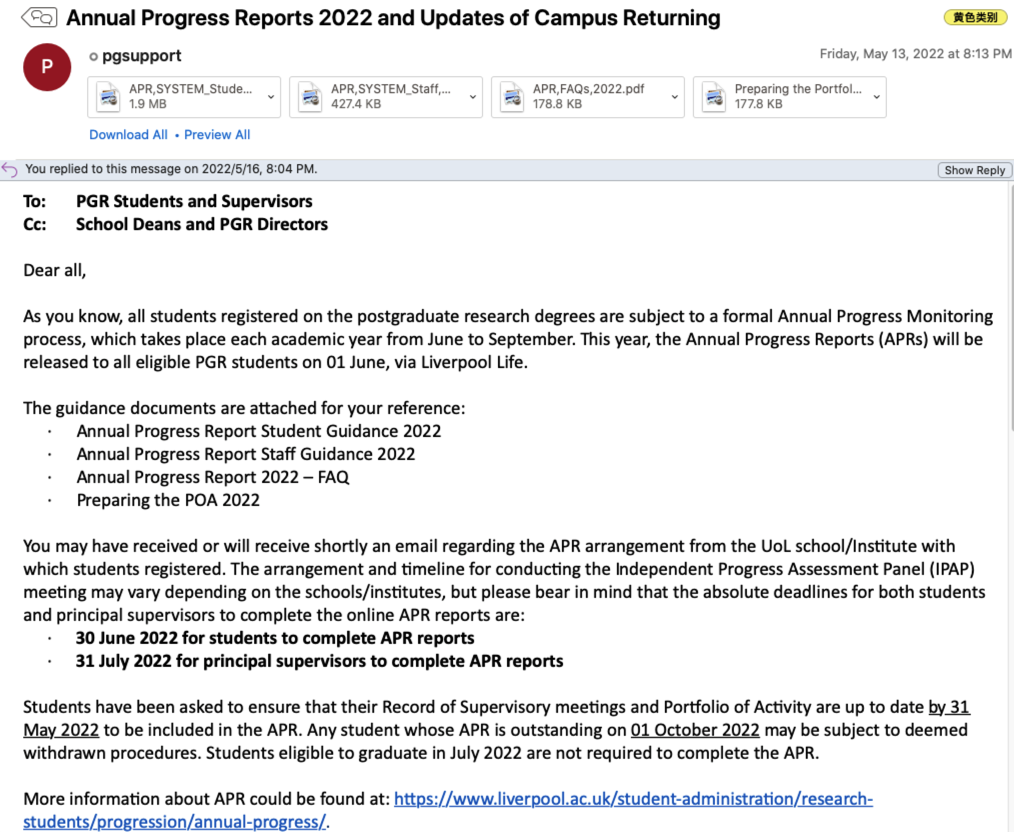
\includegraphics[width=0.5\columnwidth]{author-folder/Kai.Wu/APR_email.png}
    \end{figure}
    \item 其二为你的利物浦学院在5月发的邮件,数学学院的大概长这样,发到利物浦邮箱。其他学院的可能不太一样
    \begin{figure}[H]
        \centering
        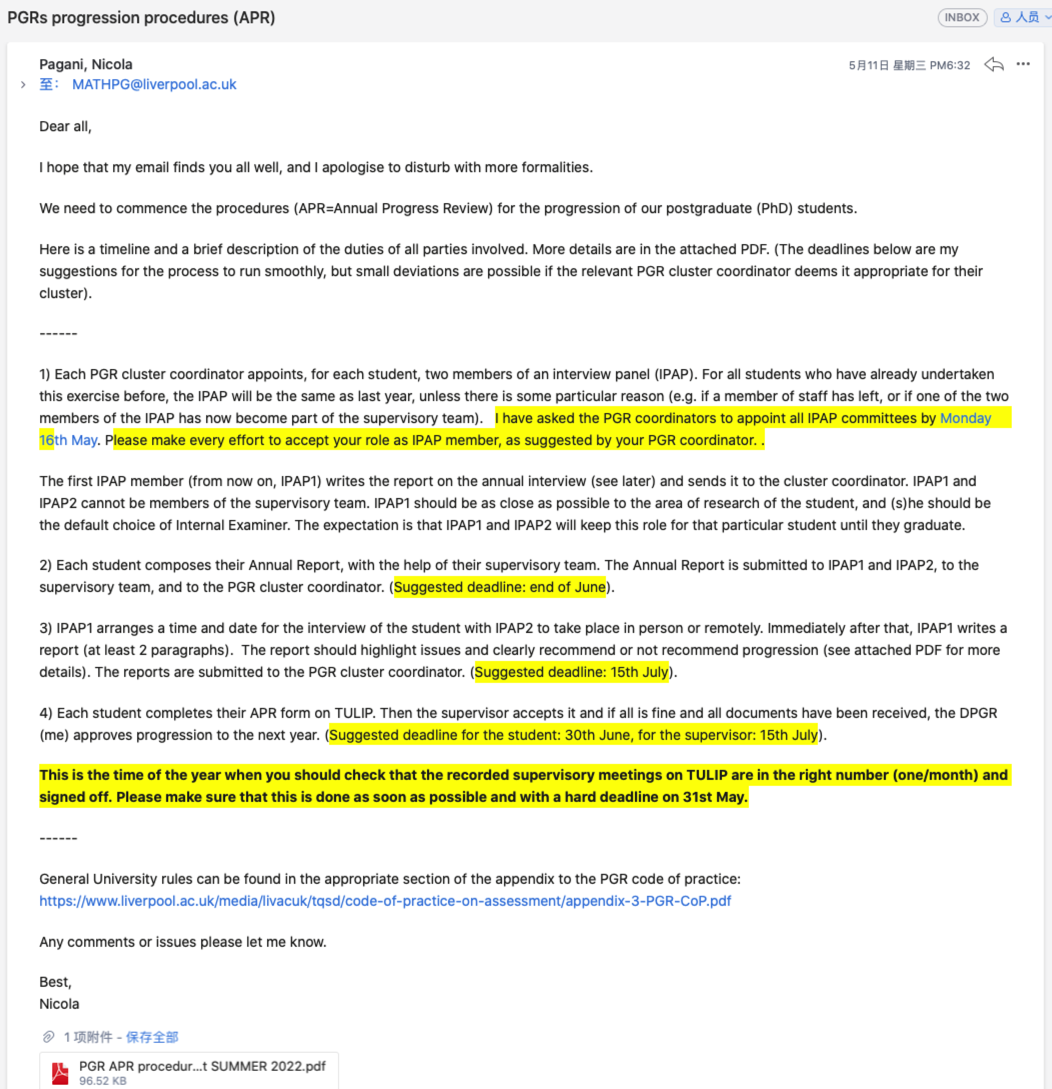
\includegraphics[width=0.5\columnwidth]{author-folder/Kai.Wu/APR_liverpool_email.png}
    \end{figure}
\end{enumerate}

每个学院的APR要求略有区别,所以在5月左右,请务必查收你的利物浦邮箱。两封邮件,特别是新生,请务必仔细阅读,特别是附件内容,\textbf{初次做APR建议对两封邮件和附件,逐字阅读}。

APR的具体内容就是下面三个部分
\subsubsection{Annual Report (AR) 年度进度报告}
简单来说,把你做了什么\textbf{写成一篇文档}。一般会有字数或者页数要求。如果你不知道些什么,我个人建议可以事无巨细的写,甚至可以写流水账。比如,读了什么文献,有了什么收获;写了什么代码/做了什么实验。以及很重要的,参加了什么学术活动,比如参加conference, meeting,还有做学校的TA,都可以写进去。
\subsubsection{Annual Seminar 年度研讨会}
一般是把一个学院或者一个系的所有PhD拉到一起做个展示,互相提提意见,了解下。但据我所知,有的人少的系和学院直接跳过了这一部分,或者把这一部分融合到下面的面试里,变成给两位老师讲。不管是什么形式,你需要\textbf{做一个PPT},让别人了解你的研究。
\subsubsection{IPAP Interview 面试}
学院会找两位不是你的导师且和你没有利益冲突的老师来和你面谈。你可能需要\textbf{做一个PPT},在里面放心大胆写下你遇到的问题。由于你的导师团队被禁止接触这一部分,所以你可以畅所欲言,以下问题都可以写。按照要求,两位老师会竭尽所能帮你解决问题
\begin{itemize}
    \item 设备问题:学校电脑故障,比如哪里用起来不顺手,卡顿,死机;办公室环境问题(例如空调对着头吹)
    \item 实实在在的科研问题:你文献读得太少,但又不知道怎么高效读;你不知道实验方法;你写作有很大困难;你因为非主观的原因无法参加很多学术会议(比如这几年,每年APR我们都要吐槽疫情的各种影响)等等
    \item 导师问题:你导师压榨你,每天让你996工作,让你疲惫不堪;你导师让你做很多无关工作,比如给他搬家,给他拿外卖,给他报销;你导师对你很凶,对你很push,让你每天精神高度紧张;你导师频繁在非工作时间打电话、发微信、邮件并要求你立即回复,让你无法休息;你导师抢你论文一作;你导师长期失联,动不动就三五天不回你邮件。这些问题,其实都是导师的严重失职。一旦遇到,都可能造成很严重的心理负担,并影响后面的工作效率。IPAP就是来做这个的,请务必和面试的老师聊清楚。
    \item 情绪、心理问题:焦虑、紧张、失眠、抑郁倾向
    \item 家庭压力:你家里要求你3年毕业,但是你觉得压力太大
    \item 经济问题,身体问题(哪里严重不舒服,可能需要休学/请假休养),等等任何影响你正常PhD工作的问题
\end{itemize}

\vspace{5mm}
定位并解决所有问题,然后开启下一学年的学习,就是APR的主要目的。如果有任何APR不方便/无法解决的问题,请及时与导师、系主任、院长、你的DA、学校的免费心理咨询室沟通。


\begin{flushright}
(2022年10月12日 by Kai Wu)
\end{flushright} \clearpage

\section{Research Symposium}

\subsection{XPGRS是什么}
XJTLU Postgraduate Research Symposium,简称XPGRS,或者Symposium,官方中文名是“博士生论坛”,是研究生院组织的活动。每年12月,会让全校的博士生一起用poster或者oral presentation展示自己的研究成果或者进展。每年的XPGRS,会在国庆节前后用邮件通知大家。

\subsection{我需要参加哪一项?}

官方要求是这样的:

\begin{itemize}
    \item 二年级的博士生需要做海报演讲
    \item 三年级的博士生需要做口头报告
    \item 四年级或以上的博士生将被邀请担任会议主席
    \item 也欢迎处于毕业论文阶段的硕士生参加
\end{itemize}

结合往年的实际情况,翻译过来就是:

\begin{itemize}
    \item 一年级的没事,但可以考虑做志愿者(会发邮件招募),或者直接去现场围观,了解前辈的工作
    \item 二年级的,必须做poster
    \item 三年级的,必须做oral presentation,可以考虑做chair
    \item 四年或以上就随便了
\end{itemize}

判断自己是哪一年级的,以当年12月1日为准。这对3-9月入学的不难,但有很多同学就恰好是在12月1日入学的。据22年的消息,这部分同学是需要做的,也就是比如21年12月入学,22年需要做poster。
% 这部分同学在一年后可以自己选择做不做。例如
% \begin{itemize}
%     \item 奥观海同学,20年12月入学。在21年12月,他发现自己做的东西太少,实在是展示不出来,于是决定不参加。这样,他在22年12月必须做poster,23年12月必须做oral presentation,24年就没事了。
%     \item 川建国同学,20年12月入学。21年12月她觉得还算可以展示一下,以及想尽早锻炼下能力,也算是为后面一年可能参加的学术会议做准备。于是她21年12月参加了poster,22年12月则必须做oral presentation,23年就没事了。
% \end{itemize}
%
当然,由于12月入学同学确实特殊,政策可能会变,因此最好每年发邮件(或者打电话)问研究生院。

理论上,其实每年你都可以同时参加poster和oral,只要你愿意!甚至,也可以从来都不去!但需要导师同意。一般没有特殊原因,导师也是希望你去锻炼下的。如果实在有原因,需要导师和研究生院联系,同意了就可以不去。(我听说过有的导师觉得symposium没卵用直接让学生从来都不参加,也有的导师,第一次就让学生同时做poster+oral...)

\begin{figure}[H]
    \caption{2021 Symposium 的 poster 会场(CB G13W),正式开始前夕}
    \centering
    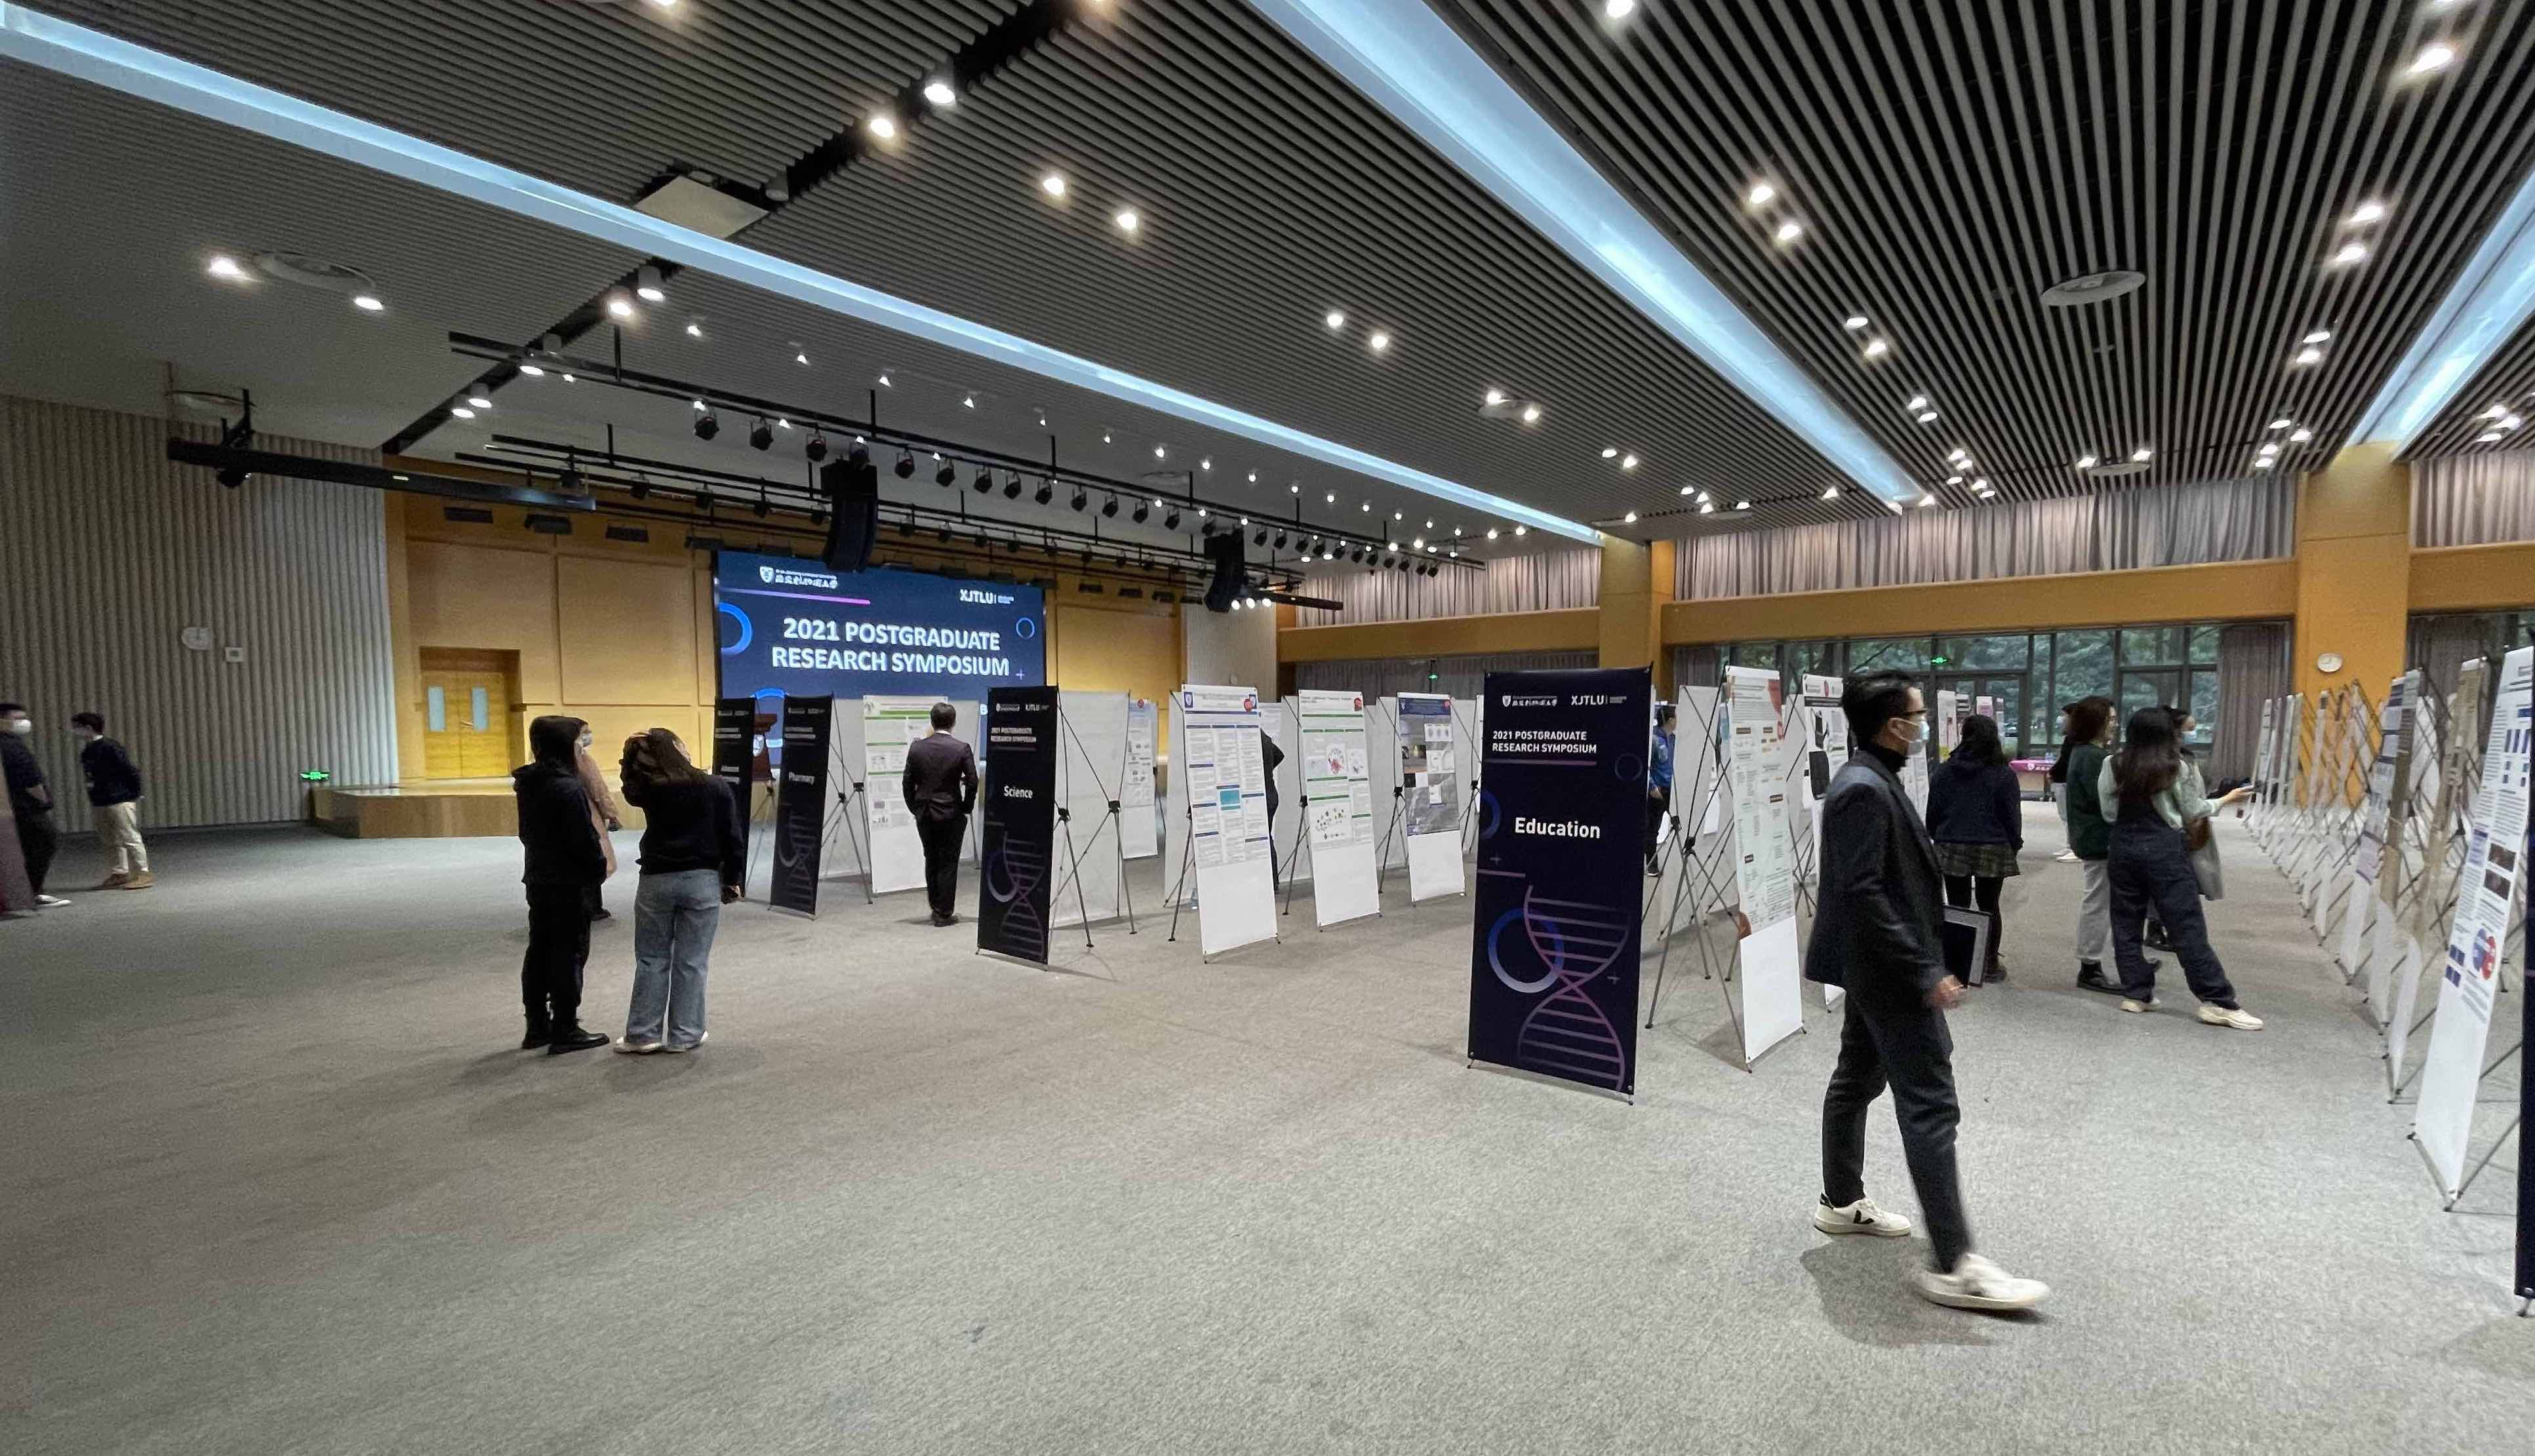
\includegraphics[width=\columnwidth]{author-folder/Kai.Wu/synposium_poster.jpg}
\end{figure}

\subsection{有什么用}

\begin{enumerate}
    \item 锻炼作报告的能力,锻炼英语口语,获得校内其他老师的指导
    \item 可以得奖。学校会请几位老师来听你讲海报、讲PPT,并给你打分。会选出最佳海报奖(10\%)最佳演讲奖(10\%)优秀海报奖(20\%)优秀演讲奖(20\%),会有一张奖状,外加1000和500元的……会议经费(会议经费使用参见章节\ref{sec.fund}),虽然不是现金奖励,但还算有用吧\sout{(抠门学校)}
\end{enumerate}

\begin{figure}[H]
    \centering
    
\includegraphics[width=0.4\columnwidth]{author-folder/Kai.Wu/poster_award.jpg}
\end{figure}

\subsection{“我不想去”——尽量不要!}

经常听到有同学这么想:奖励这么少,含金量又低,即使最后拿个最佳也没卵用。而且即使不去,最后也没能把我怎么样。是的,坦白了讲,一来,导师同意,就可以合法不去;二来,即使直接装消失,最后也不会怎么样,和毕业无关。

但,作为参加过poster、oral,也chair过三场oral、听过很多口头报告的老人,除非你作报告真的可以信手拈来,我真的强烈建议你们去参加!我见过有同学全程低头念稿,有同学直接把稿子写PPT上读,有同学过于紧张手和声音都抖个不停,有同学PPT分不清楚主次、重点不突出,有同学面对老师的问题手足无措。这些任何一项,放到你毕业答辩,都是致命的!!须知,咱答辩不是和体制内大学一样走个过场,是真枪实弹的必须要做好报告、再回答好每一个尖锐的问题。\textbf{你想要把这些问题直接暴露在答辩上,还是提前发现,多加锻炼,早些解决?}

所有,既然在Symposium里,你不会Fail,只会评奖,评委老师也都很友善,会帮你找出重要问题。所以,\uline{\textbf{是非常安全的、绝佳的【锻炼机会】}}。可不能等到答辩了或者等到你参加顶会了再去锻炼啊!

\subsection{注意事项、如何表现出色}

下面附上我在2022年symposium看到的口头报告打分表(可放大查看),poster的注意事项其实很类似(参加poster的,也需要准备一个3分钟左右的talk来给到场的评委老师介绍)。坦白的说,这些项目放在任何报告里都是值得注意的地方,可以用来仔细审视自己的海报。

\begin{figure}[H]
    \caption{2022年的打分表}
    \centering
    \begin{tabular}{rl}
        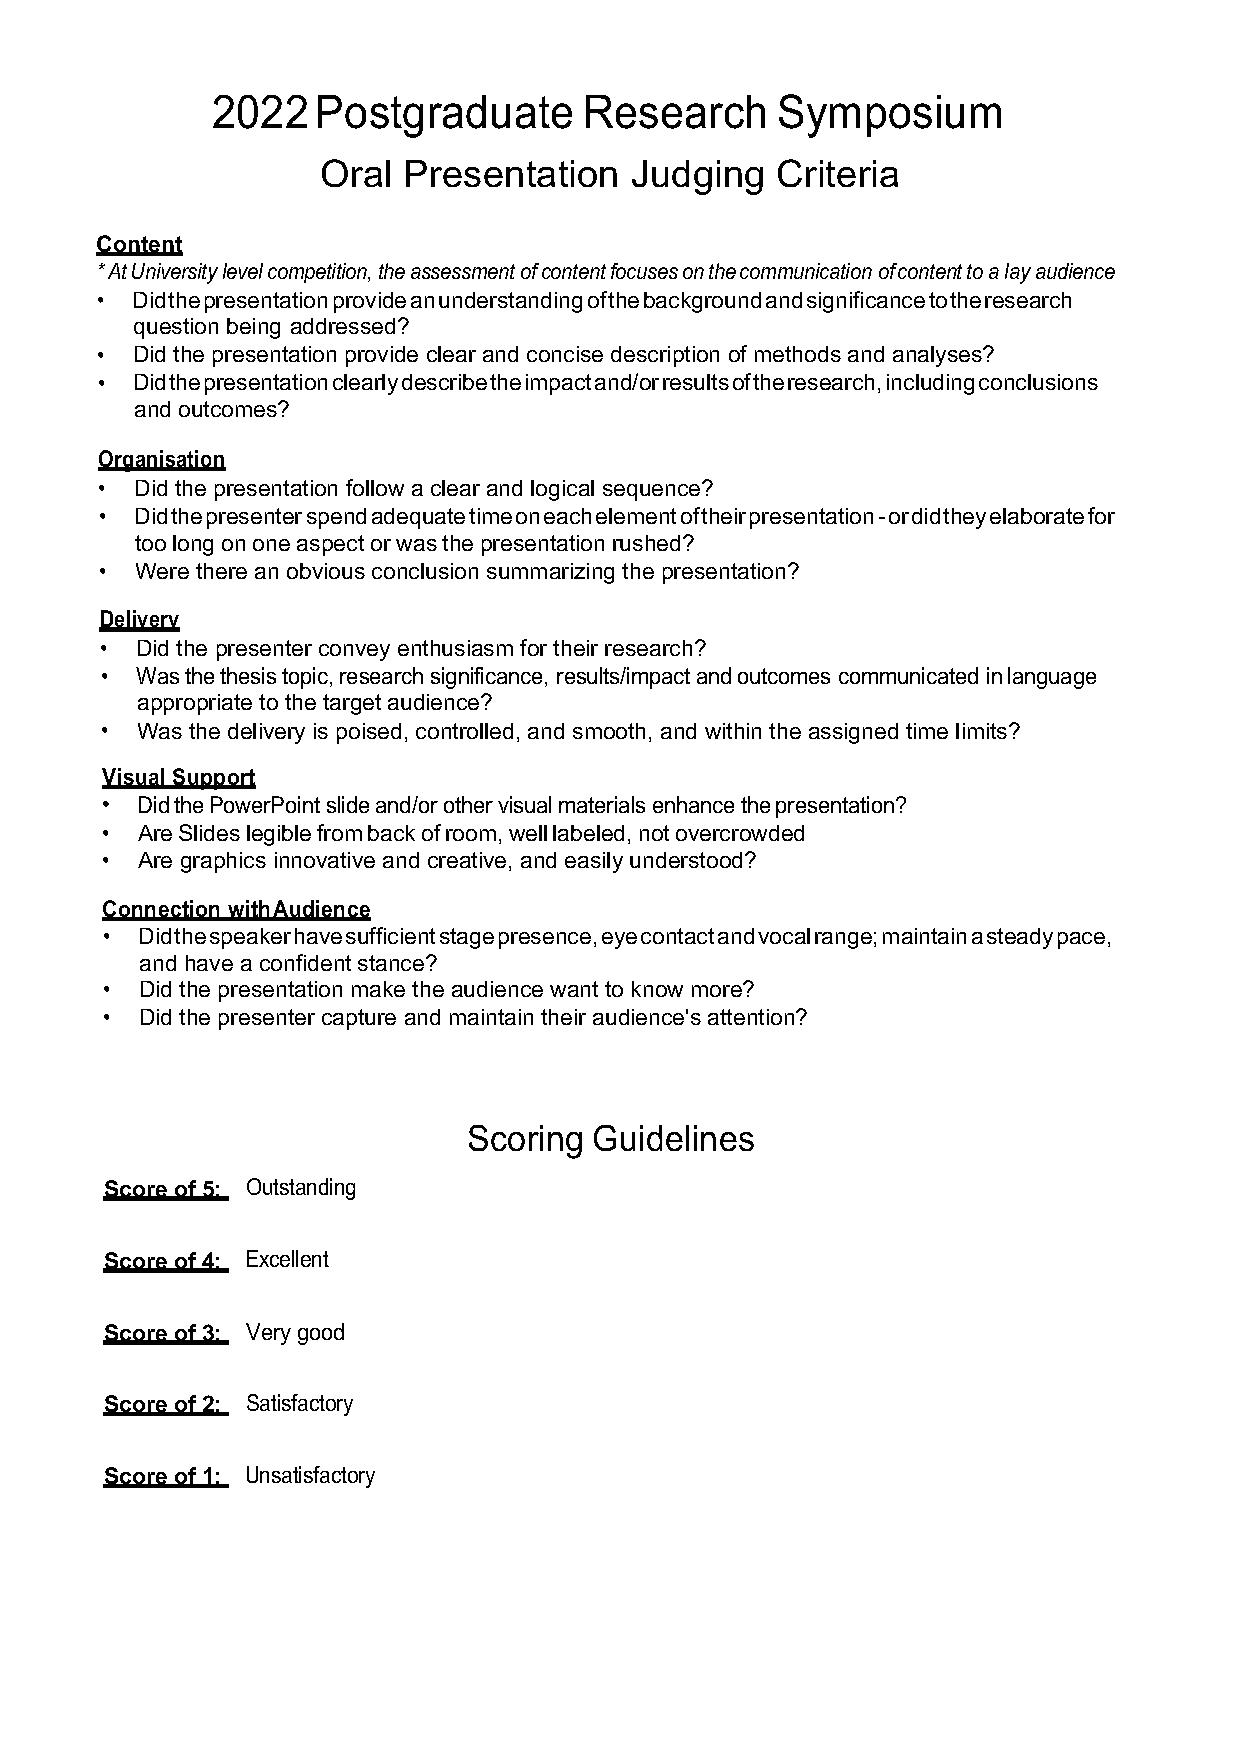
\includegraphics[width=0.5\columnwidth]{author-folder/Kai.Wu/2022_XPGRS_oral_judging_criteria.pdf} & 
        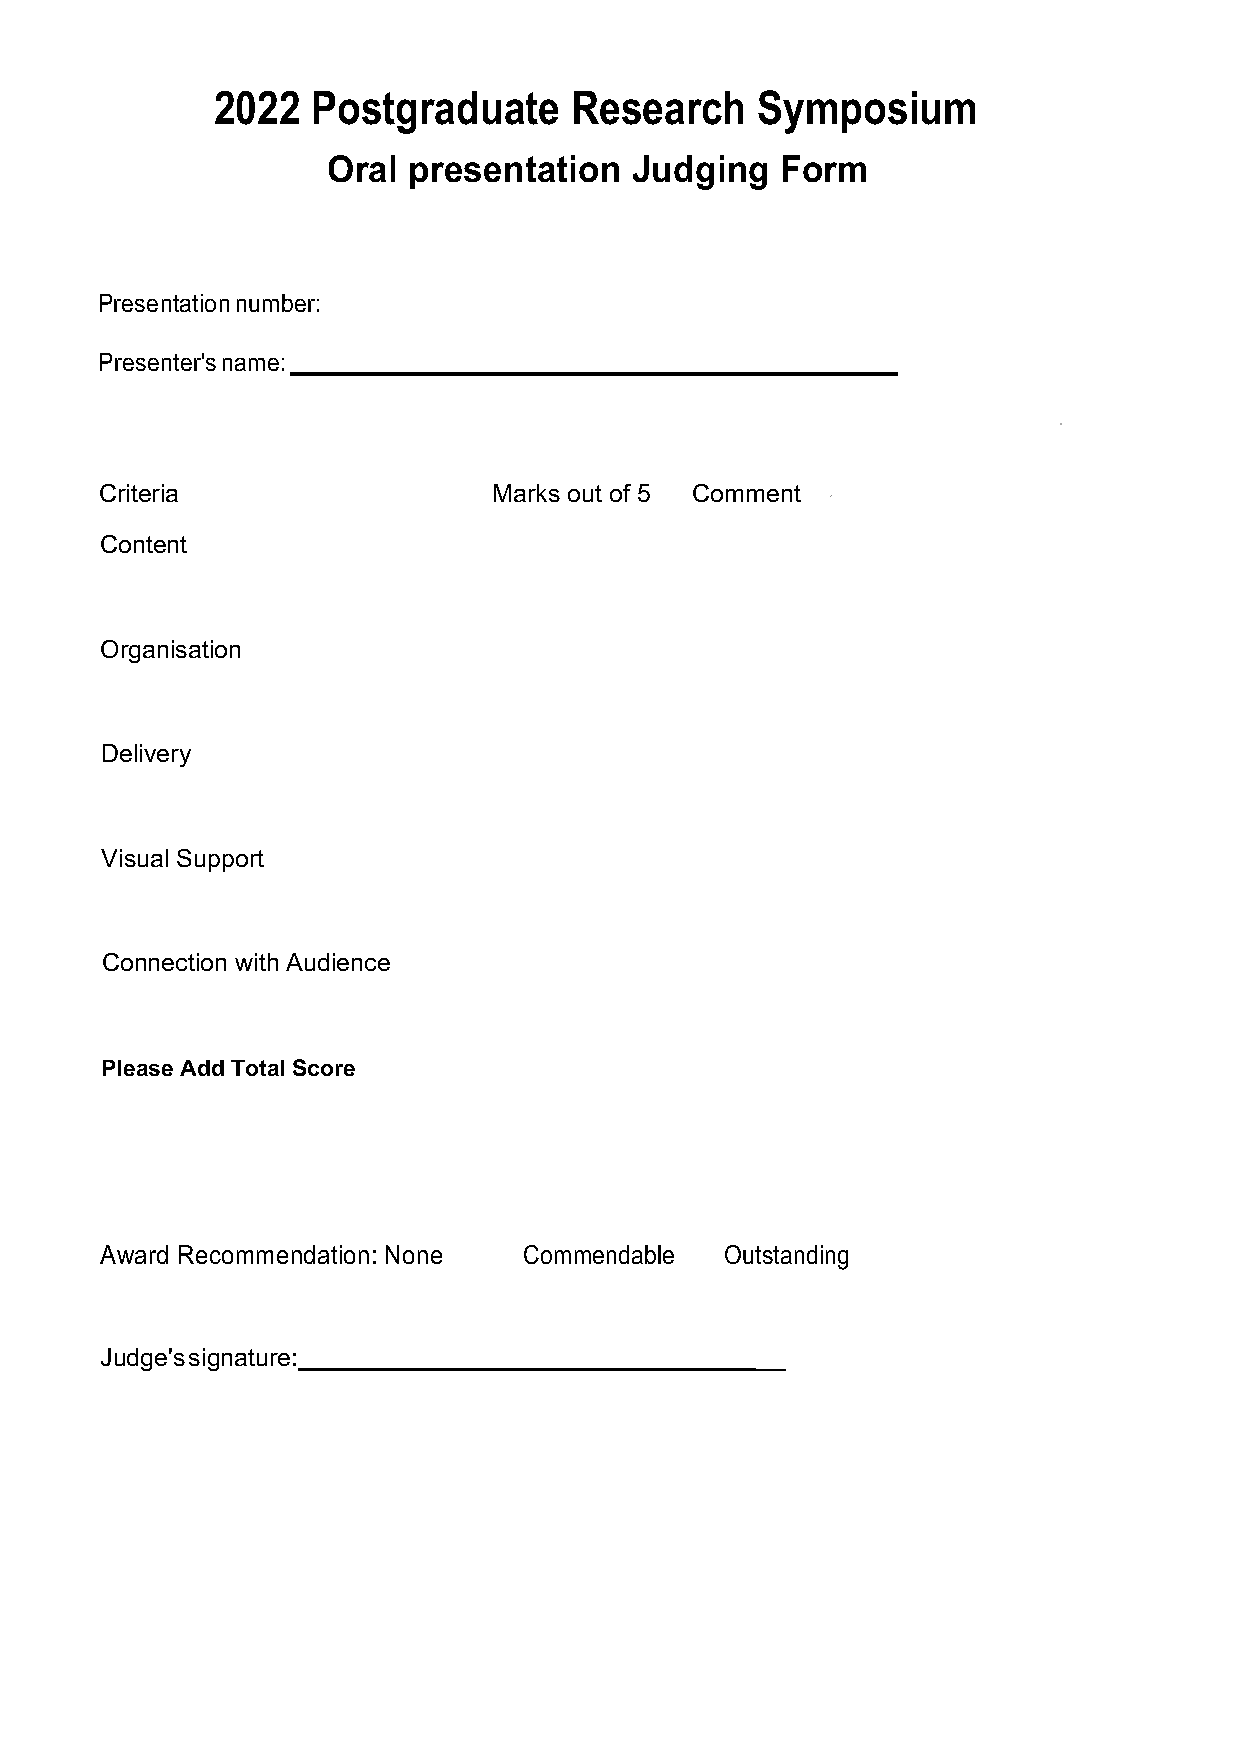
\includegraphics[width=0.5\columnwidth]{author-folder/Kai.Wu/2022_XPGRS_oral_judging_form.pdf} 
    \end{tabular}
\end{figure}

如果你想表现出色、得奖,可以继续看下面的内容:

作报告和做海报,大家在网上都能搜到大量教程。但,XPGRS和其他学术报告最大的区别就是,绝大多数同学、包括学校的评审老师,非常有可能完全不知道你的研究领域(正所谓,隔行如隔山)。如果你按照跟你导师汇报的方式来讲,或者是把你在某次内行齐聚的学术会议上的海报/PPT原封不动拿来用,有可能是得不了奖的,因为,评委老师和其他同学确实听不懂。

我的导师告诉我,XPGRS因为是给外行讲,和学术报告其实不同,更偏向科普性质。如何在短时间内,让一个外行对你的研究感兴趣,并且搞懂个70\%,也是Symposium的部分目的。如果你不知道该怎么做,可以想象有一天你在电梯里遇到了席酉民,怎么在短时间内让他知道你在做什么,又有什么用,最好还能让他感兴趣。或者是,过年回家跟你哪个亲戚或者老同学怎么讲清楚你在做什么。学术不是闭门造车,如何把自己的学术讲出去,让学术成果造福其他人也是很重要的技能。

\begin{flushright}
(2022年10月19日 by Kai Wu)

(major update: 2022年12月16日 by Kai Wu)
\end{flushright}


%# -*- coding: utf-8-unix -*-
%%==================================================

\chapter{这些必须得看,不看吃大亏}
\label{fuli}

\section{会议经费}

每位同学,无论是自费生还是奖学金学生,都有16500元的会议经费。参加会议的时候,可以用来报销注册费、住宿交通等费用。这笔钱毕业前不用完拿去\sout{在会议周边吃喝玩乐出去浪}丰富自己的学术经历就亏啦。钱虽多,申请和报销流程比较繁琐。主要资料在:
\begin{itemize}
    \item e-bridge: \url{https://ebridge.xjtlu.edu.cn/},登陆过后点击PGR Policies, Procedures and Forms,找到 \textit{Postgraduate Research Students' Conference Fund Policy} 和 \textit{
    Guideline and Procedures on Doctoral Student Travel Arrangement and Reimbursement}
    \item 官方流程图
    \begin{figure}[H]
        \centering
        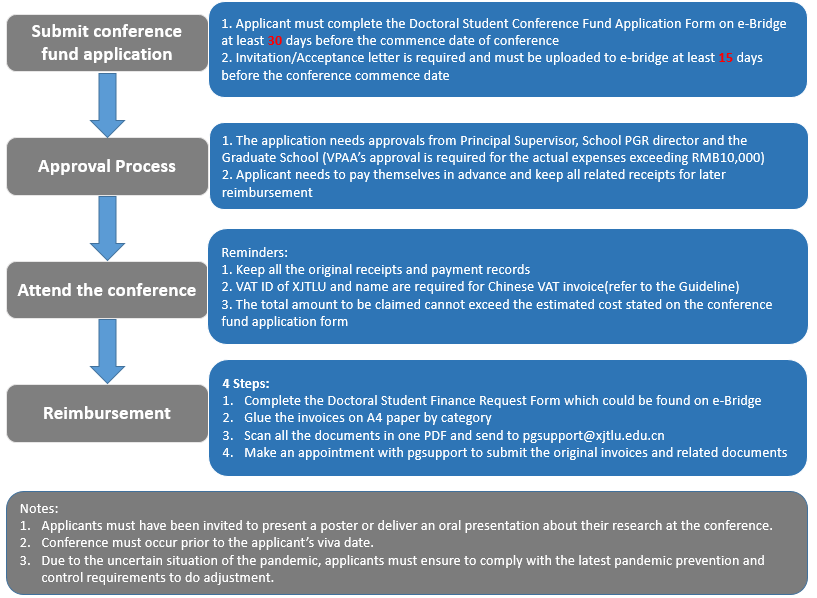
\includegraphics[width=0.9\columnwidth]{author-folder/Kai.Wu/fund-flowchart.png}
    \end{figure}
\end{itemize}

要注意
\begin{enumerate}
    \item 必须要至少提前30天申请。因此不能用于“你突然听说有个30天内要开的会议”
    \item 必须要在会议上作报告,poster或者oral都可以,否则不能使用经费
    \item 不能使用学校经费的时候,可能可以使用你导师的某些经费。我就因为上述原因,用导师的经费报销过几场会议。具体怎么做\&你导师到底有没有这种经费,问你自己的导师
\end{enumerate}


\begin{flushright}
(2022年10月12日 by Kai Wu)
\end{flushright}
\section{免费办公用品}
\begin{figure}[H]
    \centering
    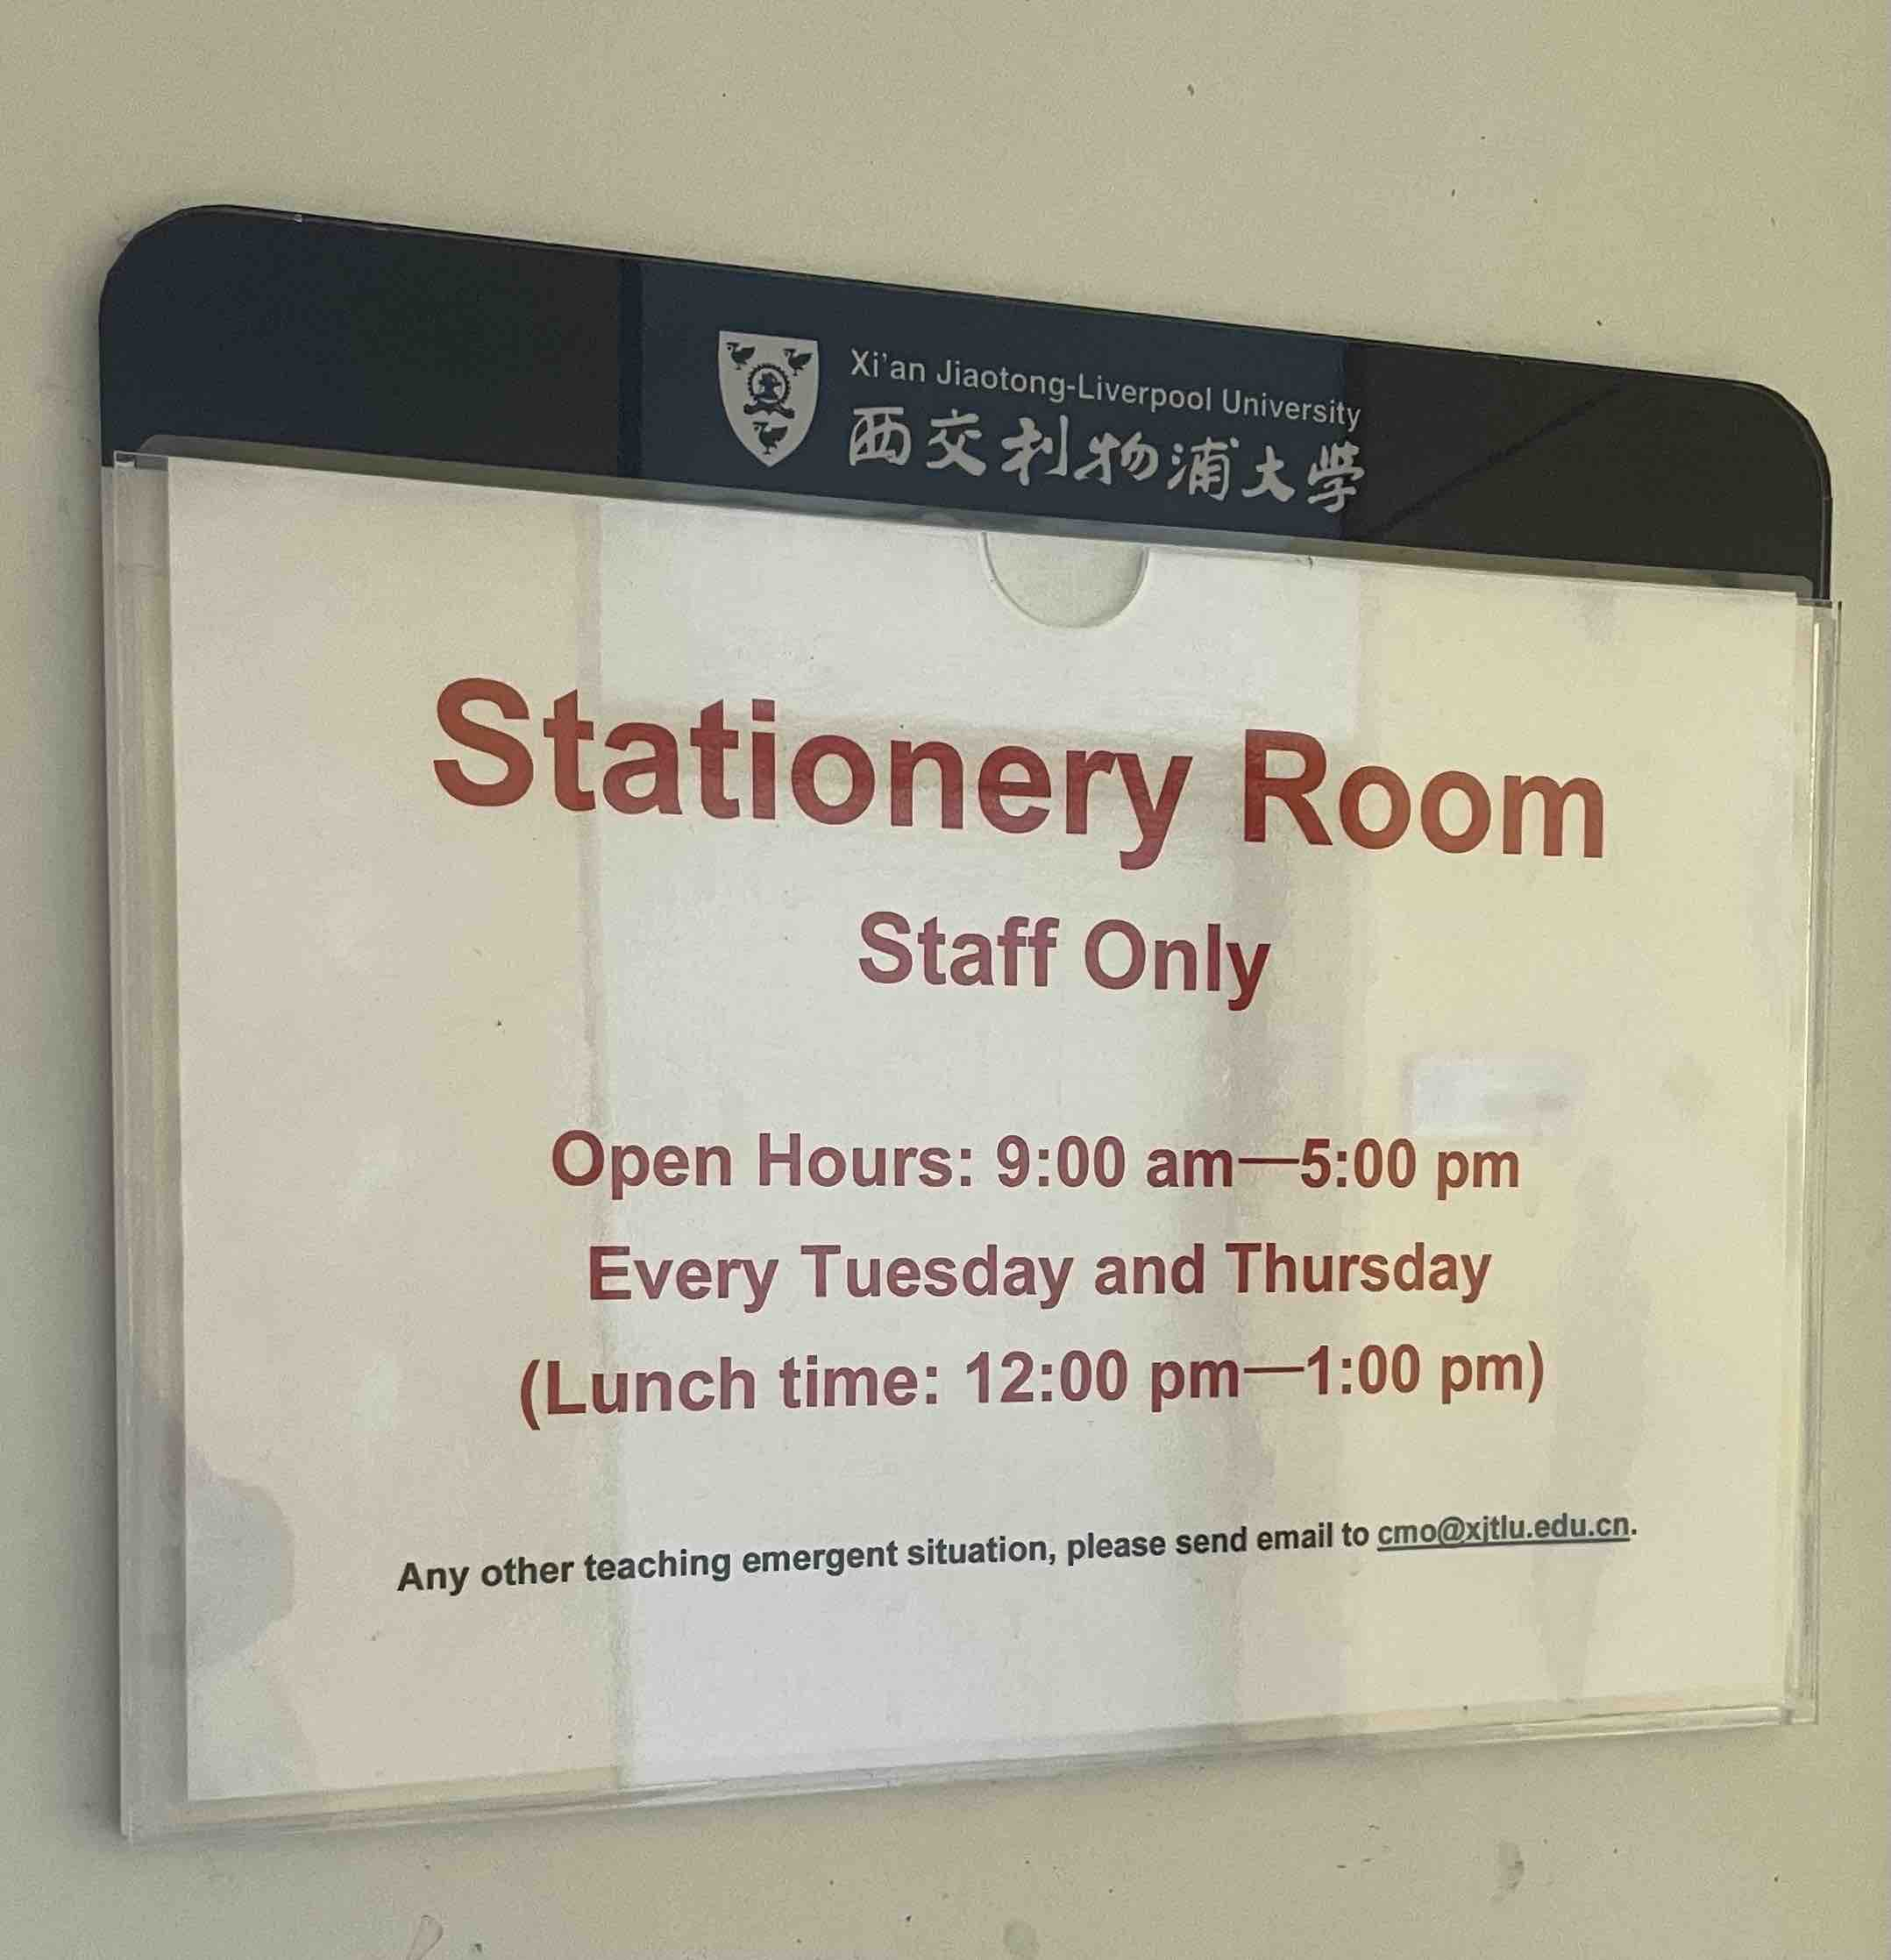
\includegraphics[width=0.6\columnwidth]{author-folder/Kai.Wu/stationery_room.jpg}
\end{figure}

除了大笔的会议经费之外,最让大家省钱的应该就是免费的办公用品了。学校很多楼里都有Stationery room(办公用品领用室),里面所有东西都可以领取。抽纸、笔、马克笔、荧光笔、各种收纳架子、胶带胶水订书机,基本你能想到的都有。

\vspace{5mm}
哪些地方有stationery room:
\begin{itemize}
    \item MB一楼,每周二/周四,上午9-11点,下午1-5点
    \item BS一楼(房间号?谁知道房间号来补充下)(开放时间?)
    \item 其他楼?请读者补充
\end{itemize}

\vspace{5mm}
如何领取:
\begin{enumerate}
    \item 第一次领取前,先直接跑到stationery room,问工作人员可以领哪些,ta会给你一个册子。拍照留存每一页内容,这样下次就知道可以拿什么了
    \item 下载最新的 (CMO) Office Supplies Application Form,目前最新版本是V3。新版本发布后老版本一般是不能用的。如果这个过期了,更新的版本我们在哪里下载呢?很遗憾我们没法下载,一般方法是,问你导师要,导师一般可以在学校的box网盘里面找到。这里提供一个我在用的 \url{https://cowtransfer.com/s/e7089cbffe9c43},也可在本项目的GitHub里(\href{https://github.com/kaiwu-astro/xp_pgrs_unofficial_guide/tree/main/fileshare}{链接})找到。
    \item 如实填写内容。其中第一列[办公用品名称]一定要和上面那个册子里的物品名称一样。每次不能拿太多,拿东西的工作人员会审查。抽纸每次只能拿一盒。笔一般是按支拿,不能按盒拿(但是你可以写拿12支,就是1盒)。右边的理由,如实简单填写,比如抽纸-日用;笔-演算;订书机-整理;胶水-报销。最后,要你导师签字。电子签名应该不能用,也不能导师签完过后复印(这些都是之前版本常用的花招hhh)。
\end{enumerate}


\begin{flushright}
(2022年10月12日 by Kai Wu)
\end{flushright}
\section{免费打印}
每个9月,学校都会把博士生的打印费余额重置为2000元(可在 \url{https://myprint.xjtlu.edu.cn} 查询),相当于,每位博士生同学有几乎无限制的打印费。我个人就喜欢把论文全部打出来看。
如何打印,建议直接看官方文档。文件在本项目的GitHub里(\href{https://github.com/kaiwu-astro/xp_pgrs_unofficial_guide/tree/main/fileshare}{链接}),或者下面的链接
\begin{itemize}
    \item 本科生IT指南(中英文):\url{https://cowtransfer.com/s/c2a6a246e31a4e}
    \item 打印指南(英文):\url{https://guide.xjtlu.edu.cn/ss-print/staff}
\end{itemize}

注意,请不要用于打印整本书籍,这违反打印政策,可能会被查,但打书的个别章节一般是允许的。如果一定要打整本书,请淘宝。


\begin{flushright}
(2022年10月12日 by Kai Wu)
\end{flushright}
\section{体育馆代金券}


\begin{flushright}
( by Kai Wu)
\end{flushright}
\section{利物浦账号自带福利}
\begin{itemize}
    \item Liverpool 免费高级Zoom账户:\url{https://liverpool.service-now.com/sp?id=kb_article&sysparm_article=KB0011854}
    \item Liverpool 免费 Office365:\url{https://liverpool.service-now.com/sp?id=kb_article&sysparm_article=KB0010032}
    \item Liverpool 免费 1T Onedrive 云盘 网页使用: \url{https://liverpool.service-now.com/sp?id=kb_article&sysparm_article=KB0011362}
    \item Liverpool 免费 1T Onedrive 云盘 本地备份同步: \url{https://support.microsoft.com/zh-cn/office/%E4%BD%BF%E7%94%A8-onedrive-%E8%BF%9B%E8%A1%8C%E5%90%8C%E6%AD%A5-bb89981b-e382-4969-b8fd-d413a90b6db3}
    \item 其他Liverpool免费软件:\url{https://www.liverpool.ac.uk/it/software/software-downloads/}
    \item Liverpool软件序列号:\url{https://www.liverpool.ac.uk/it/software/licencecodes/}
\end{itemize}

\begin{flushright}
    (2022年10月2日 by Kai Wu)
    \end{flushright}
\section{景区学生票(和火车票学生票)优惠}

% 传闻最新情况博士生不发学生证,本篇攻略废弃

和本科生一样,我们也是能享受学生票优惠的。步骤如下

\begin{enumerate}
    \item 申请学生证。学生证,不是你的ID卡,是红色的小本本。博士生,默认是不发学生证的,要自己申请才发。方法:在一站式网站 \url{https://studentonestop.xjtlu.edu.cn/} 里的申请/补办学生证,按提示操作。学生证可用于各景点买学生票(例如拙政园,买学生票过后进门查学生证。ID卡是不行的)。
    \item 据部分同学反应,2020年之后给博士生发的学生证没有火车票优惠卡了(最后一页上的芯片小贴纸),我不知道不发这个是否合规,具体可骚扰一站式或pgsupport。如果你的学生证没有火车票优惠卡,就不能买火车票的学生票,但景区优惠不受影响。
    \item 注意盖注册章:在景区门口(或火车上)如果遇到工作人员double check你学生身份,发现你学生证注册章不是最新的,按政策是可以要求你补全票的。所以,去景区(或坐火车)之前,要注意注册章要盖够了。我的做法是,买学生票的时候再去check自己注册章有没有盖够,否则立马去一站式补就行(可以一口气盖一堆)。
    \item 
        \begin{minipage}{0.71\textwidth}
            如果你有火车票优惠卡,可以继续看这部分:如何使用?如何购买火车票学生票?有什么限制?因为政策可能变动,请直接关注官方公众号,在公众号菜单里有常见问题FAQ。
        \end{minipage}
        \begin{minipage}{0.2\textwidth}
            \begin{figure}[H]
                
\includegraphics[width=0.95\columnwidth, center]{author-folder/Kai.Wu/qrcode_huitongstudent_1.jpg}
            \end{figure}
        \end{minipage}

\end{enumerate}


\begin{flushright}
(2023年01月04日 by Kai Wu)
\end{flushright}

% \begin{figure}[H]
%     \centering
%     \includegraphics[width=0.5\columnwidth]{author-folder/Kai.Wu/}
% \end{figure}


% \usepackage[export]{adjustbox}

% \item 

% \begin{newminipage}[0.65]
%     文字
% \end{newminipage}
% \begin{newminipage}[0.34]
%     \begin{figure}[H]
%         % \caption{}
%         \includegraphics[width=0.95\columnwidth, right]{author-folder/Kai.Wu/}
%     \end{figure}
% \end{newminipage}

% \input{author-folder/Kai.Wu/.tex}


\section{其他福利}

下面的内容,如果你完全没见过,可以花几分钟探索一下,留个印象,可能对以后很有帮助

\begin{enumerate}
    \item 学校提供的IT服务:\url{https://guide.xjtlu.edu.cn/it-guide-for-student.html}
\end{enumerate}


%# -*- coding: utf-8-unix -*-

\chapter{最好要知道这些}

\section{助教(Teaching Assistant)怎么做}

\subsection{我是否需要做TA?}
\begin{itemize}
    \item 如果你是全额奖学金的博士生(免学费+有津贴),那根据学校发给你的的Financial offer,你每学期都有TA的义务(换句话说,奖学金是TA工作量换来的,拿了钱必须做事)。做了TA过后,不会另外结算工资。2020年及之后入学的全奖博士,三年需要做满900小时助教方可毕业。
    \item 如果你是2020年及之后入学的半奖博士生(仅免学费)或者自费生,需做满500小时助教方可毕业。做TA过后,学校会按照工时给你发工资,而且TA的经历写到你简历上,(视你未来的职业规划)可能有一些作用。
\end{itemize}

\begin{flushright}
    (2022年10月21日 by Kai Wu)

    (major update: 2022年12月30日 by Yue Zhou)
\end{flushright}

\subsection{如何成为一名TA}

每学期的第一周前后,学院会招募TA,一般由学院的秘书(School Academic Administrator)联系大家。
\begin{itemize}
    \item 半奖及自费博士比较自由,可自行与任课老师联系
    \item 全奖博士分两种情况:a.自行与任课教师联系 b.学院直接发邮件分配
\end{itemize}

如果你很想参加,或者想早点占某个科目、某为老师的坑,可以尽早联系秘书以及对应的科任老师。

\begin{flushright}
    (2022年12月30日 by Yue Zhou)
\end{flushright}

\subsection{TA的工作种类,以及分别怎么做}

助教的工作包括不局限于
\begin{enumerate}
    \item 批改作业及试卷
    \item 给本硕学生上tutorial(商科居多)、上lab
    \item 核算登记课程分数
    \item 做一些辅助性的工作(如设置Learning Mall等)
    \item 期中、期末监考
\end{enumerate}

研究生院会组织TA培训,以\textit{Teaching Assistant (TA) Training Programme}为题的邮件通知,也可以直接在你的Learning Mall上找到。每学期都有。如果一次都没去过,最好至少去听一次。下面是比较核心的、学校培训讲不太明白的内容:

\subsubsection{批作业}
如果是传统的改线下的纸质作业,一般问老师怎么做就行。如果是通过Learning Mall(以下简称LMO)提交的电子版作业,下面是教程:
\begin{enumerate}
    \item 登录LMO,找到你做助教的课程。如果翻遍了都找不到,需要发邮件给你们学院的秘书或者任课老师给你权限。
    \begin{figure}[H]
        \centering
        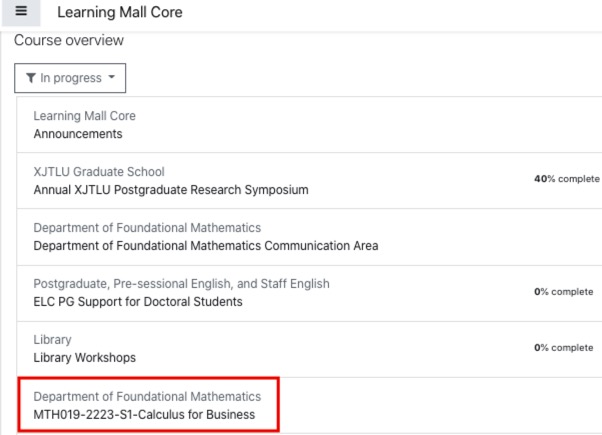
\includegraphics[width=0.4\columnwidth]{author-folder/Kai.Wu/LMO_course.jpg}
    \end{figure}

    \item 
    \begin{minipage}{0.3\textwidth}
        点进课程,往下拉找到提交作业的地方,或者直接用Ctrl+F(Mac:Command+F)搜索 submission
    \end{minipage}
    \begin{minipage}{0.63\textwidth}
        \begin{figure}[H]
            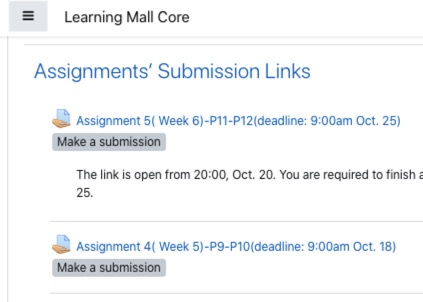
\includegraphics[width=0.95\columnwidth, right]{author-folder/Kai.Wu/LMO_submission_links.jpg}
        \end{figure}
    \end{minipage}

    \item 超大的必修课会有很多个班,先选择你被分配到改作业的班级(Seperate group)。接下来,如果你要马上开始在网页上在线批改,点击Grade。如果想看看,或者想离线批改(比如下载到iPad上),点击view all submission。
        \begin{figure}[H]
            \centering
            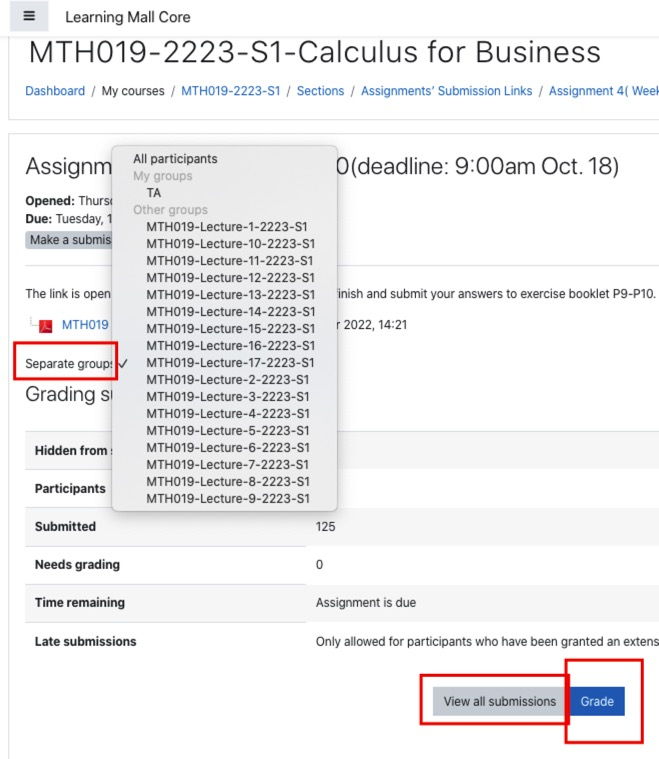
\includegraphics[width=0.5\columnwidth]{author-folder/Kai.Wu/LMO_inside_submission.jpg}
        \end{figure}
    \item 我对在线批改系统深恶痛绝,很卡,而且在线的PDF标记工具贼难用,改作业效率很低。除非老师做了打分表格(我导师给我展示过一次,在线批改的时候右边可以直接选择每个小题的分数,以及错误原因,这样就很高效,但我改过作业的module一个都没有做过这个),否则在线就很鸡肋。因此下面我只介绍我摸索出来的相对高效的离线批改方法。点进view all submission过后,在上面的grade action里,分别选择[下载成绩表]和[下载全部提交文件]
        \begin{figure}[H]
            \centering
            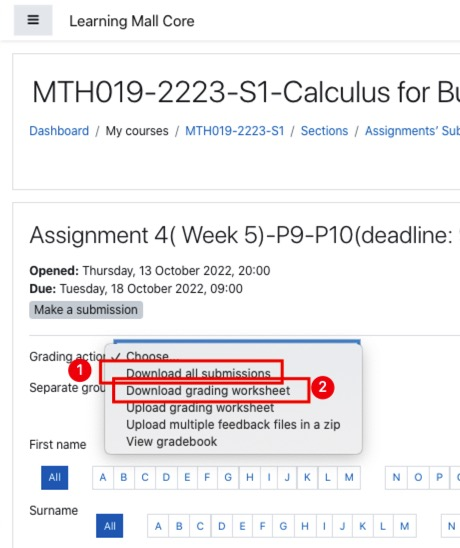
\includegraphics[width=0.5\columnwidth]{author-folder/Kai.Wu/LMO_download.jpg}
        \end{figure}
    \item 然后你就会获得一个csv文件和一个超级大zip。解压zip会看到所有学生提交的作业都以姓名+学号+一堆字命名好了。接下来你就可以把这堆文件在你电脑上、或者传到平板上本地批改。如果你的科任老师不要求把批改过的作业作为feedback file发回给学生(得问老师),你甚至可以全部打印出来改。改完过后,把成绩登到成绩表里。csv可以用Excel打开,你可以另存为xlsx格式。表格最后一列是Feedback comments,可以在里面写对学生要说的话,比如,文件格式不对、下次请拍清晰一点,之类的
        \begin{figure}[H]
            \centering
            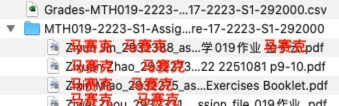
\includegraphics[width=0.5\columnwidth]{author-folder/Kai.Wu/LMO_Downloaded.jpg}
        \end{figure}
    \item 按照老师的要求改完作业过后,可以很方便的把成绩表和批改过的文件(如果老师要求)传回LMO。还是在刚才view all submission之后的页面,点击upload grading worksheet,把成绩表传上去。
        \begin{figure}[H]
            \centering
            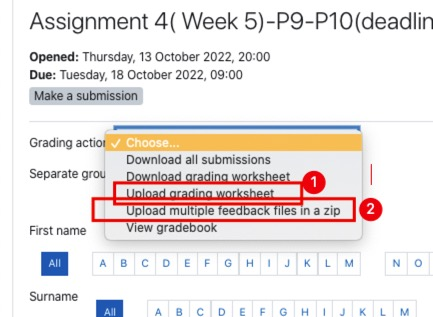
\includegraphics[width=0.5\columnwidth]{author-folder/Kai.Wu/LMO_upload.jpg}
        \end{figure}
    \item 要注意,如果你中间用Excel把它存成了xlsx,上传前需要另存为UTF-8的csv格式再上传。勾选下面allow那一句,允许表格内容覆盖已经在网页改过的内容。点击下面upload过后,你会看到很长一串网页,每个学生的成绩(和你输入的feedback comments)就传上去了。
        \begin{figure}[H]
            \centering
            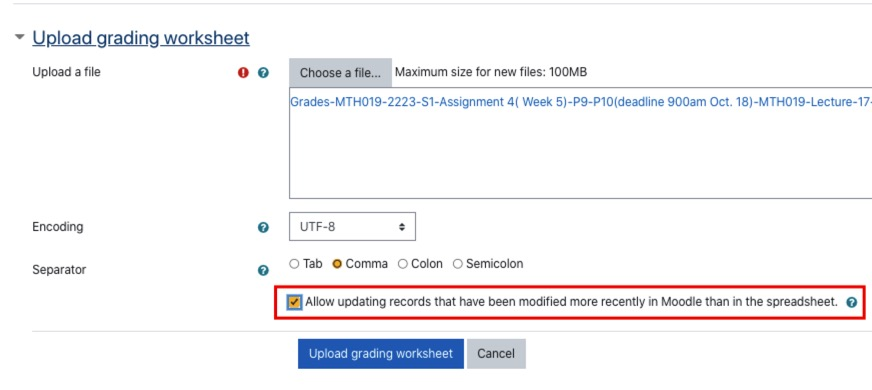
\includegraphics[width=0.8\columnwidth]{author-folder/Kai.Wu/LMO_upload_sheet.jpg}
        \end{figure}
    \item 回到刚才的页面,点upload multiple feedback files in a zip,上传批改过的作业文件。把作业文件打包成zip上传,但由于LMO限制上传大小不能超过100M,如果总大小超过了就要手动打包成多个小于100M的zip(神烦,为什么下载就可以超过100M)。会用Python的,可以用我随便写的这个Python脚本 \href{https://github.com/kaiwu-astro/xp_pgrs_unofficial_guide/tree/main/fileshare/zip_in_100M.py}{GitHub链接} 或 \href{https://cowtransfer.com/s/ca761995ed6945}{不能上GitHub的用这个链接},来自动按最大100M打包成多个文件(如果不会Python当然还是手动打包比较快)。上传完过后就完事了。
    \item 最后要发邮件给老师,说明(1)发现的共性问题,比如某道题错得很多,某道题不会的很多,某道题有的学生错理解成了什么,之类的,(2)个别问题,例如某学生交错了文件,某学生疑似抄袭标准答案(这种一般是高年级学生给他的),某学生和某学生作业雷同,(3)以及其他任何想和老师沟通的问题。大学数学系有下面这种专门的反馈表,填到表里。如果没有反馈表的,给老师发邮件说下也可以。(一般都不用太详细,不要学我,很费时间,除非你热爱这项事业)
        \begin{figure}[H]
            \centering
            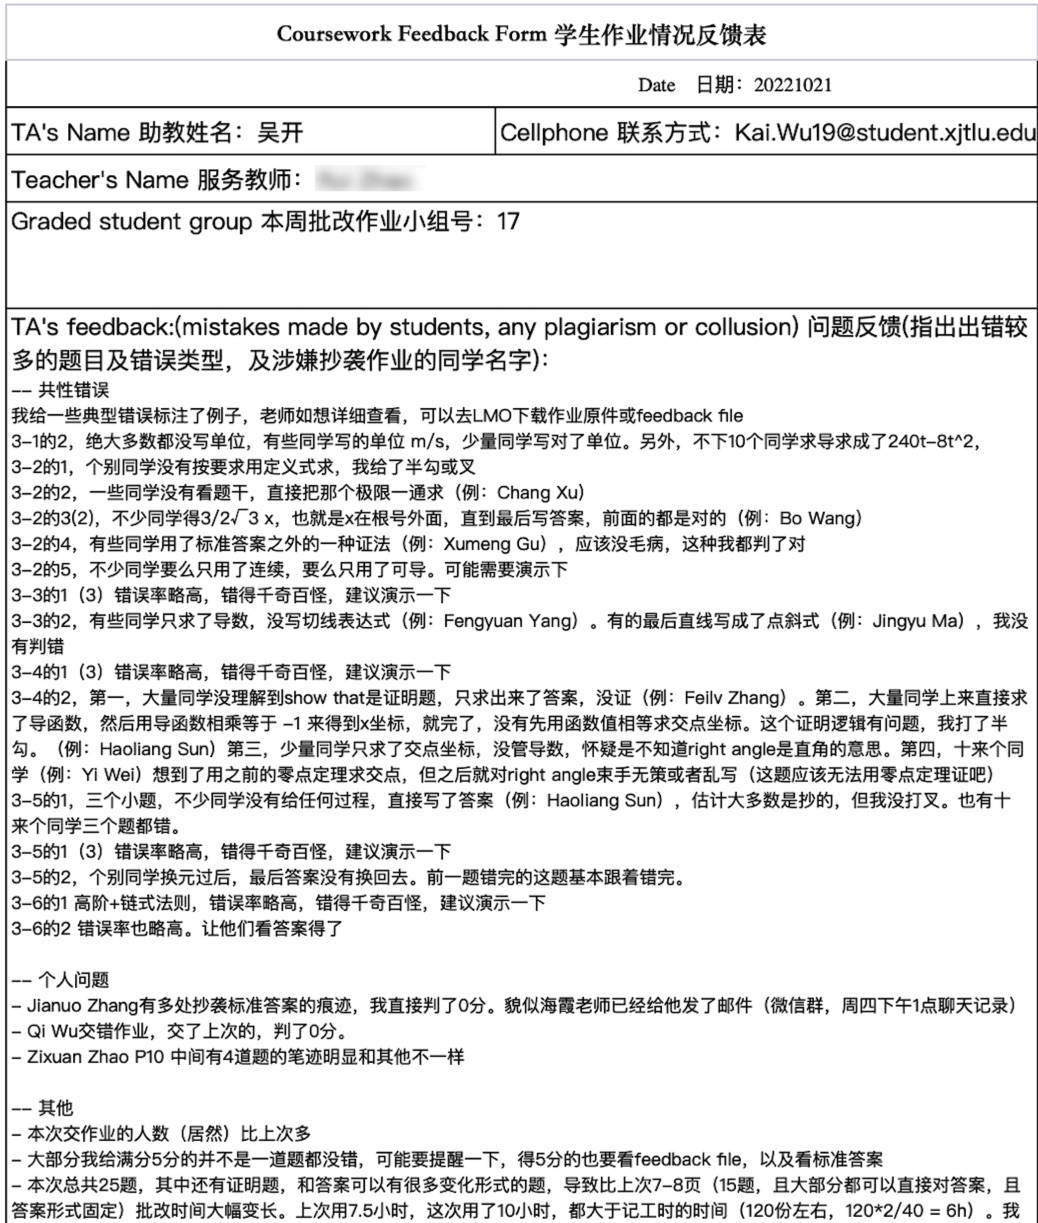
\includegraphics[width=0.5\columnwidth]{author-folder/Kai.Wu/LMO_feedback_to_teacher.jpg}
        \end{figure}
\end{enumerate}


\emptyline
【分享一下我的批作业经验】
\begin{enumerate}
    \item 我的工具组合是iPad + Apple pencil + PDF Expert app,比在电脑上在线、离线改都快得多。另外如果购买磁吸类纸膜(约20元)+ pencil替换笔头(约10元),会大幅提高书写体验
        \begin{figure}[H]
            \centering
            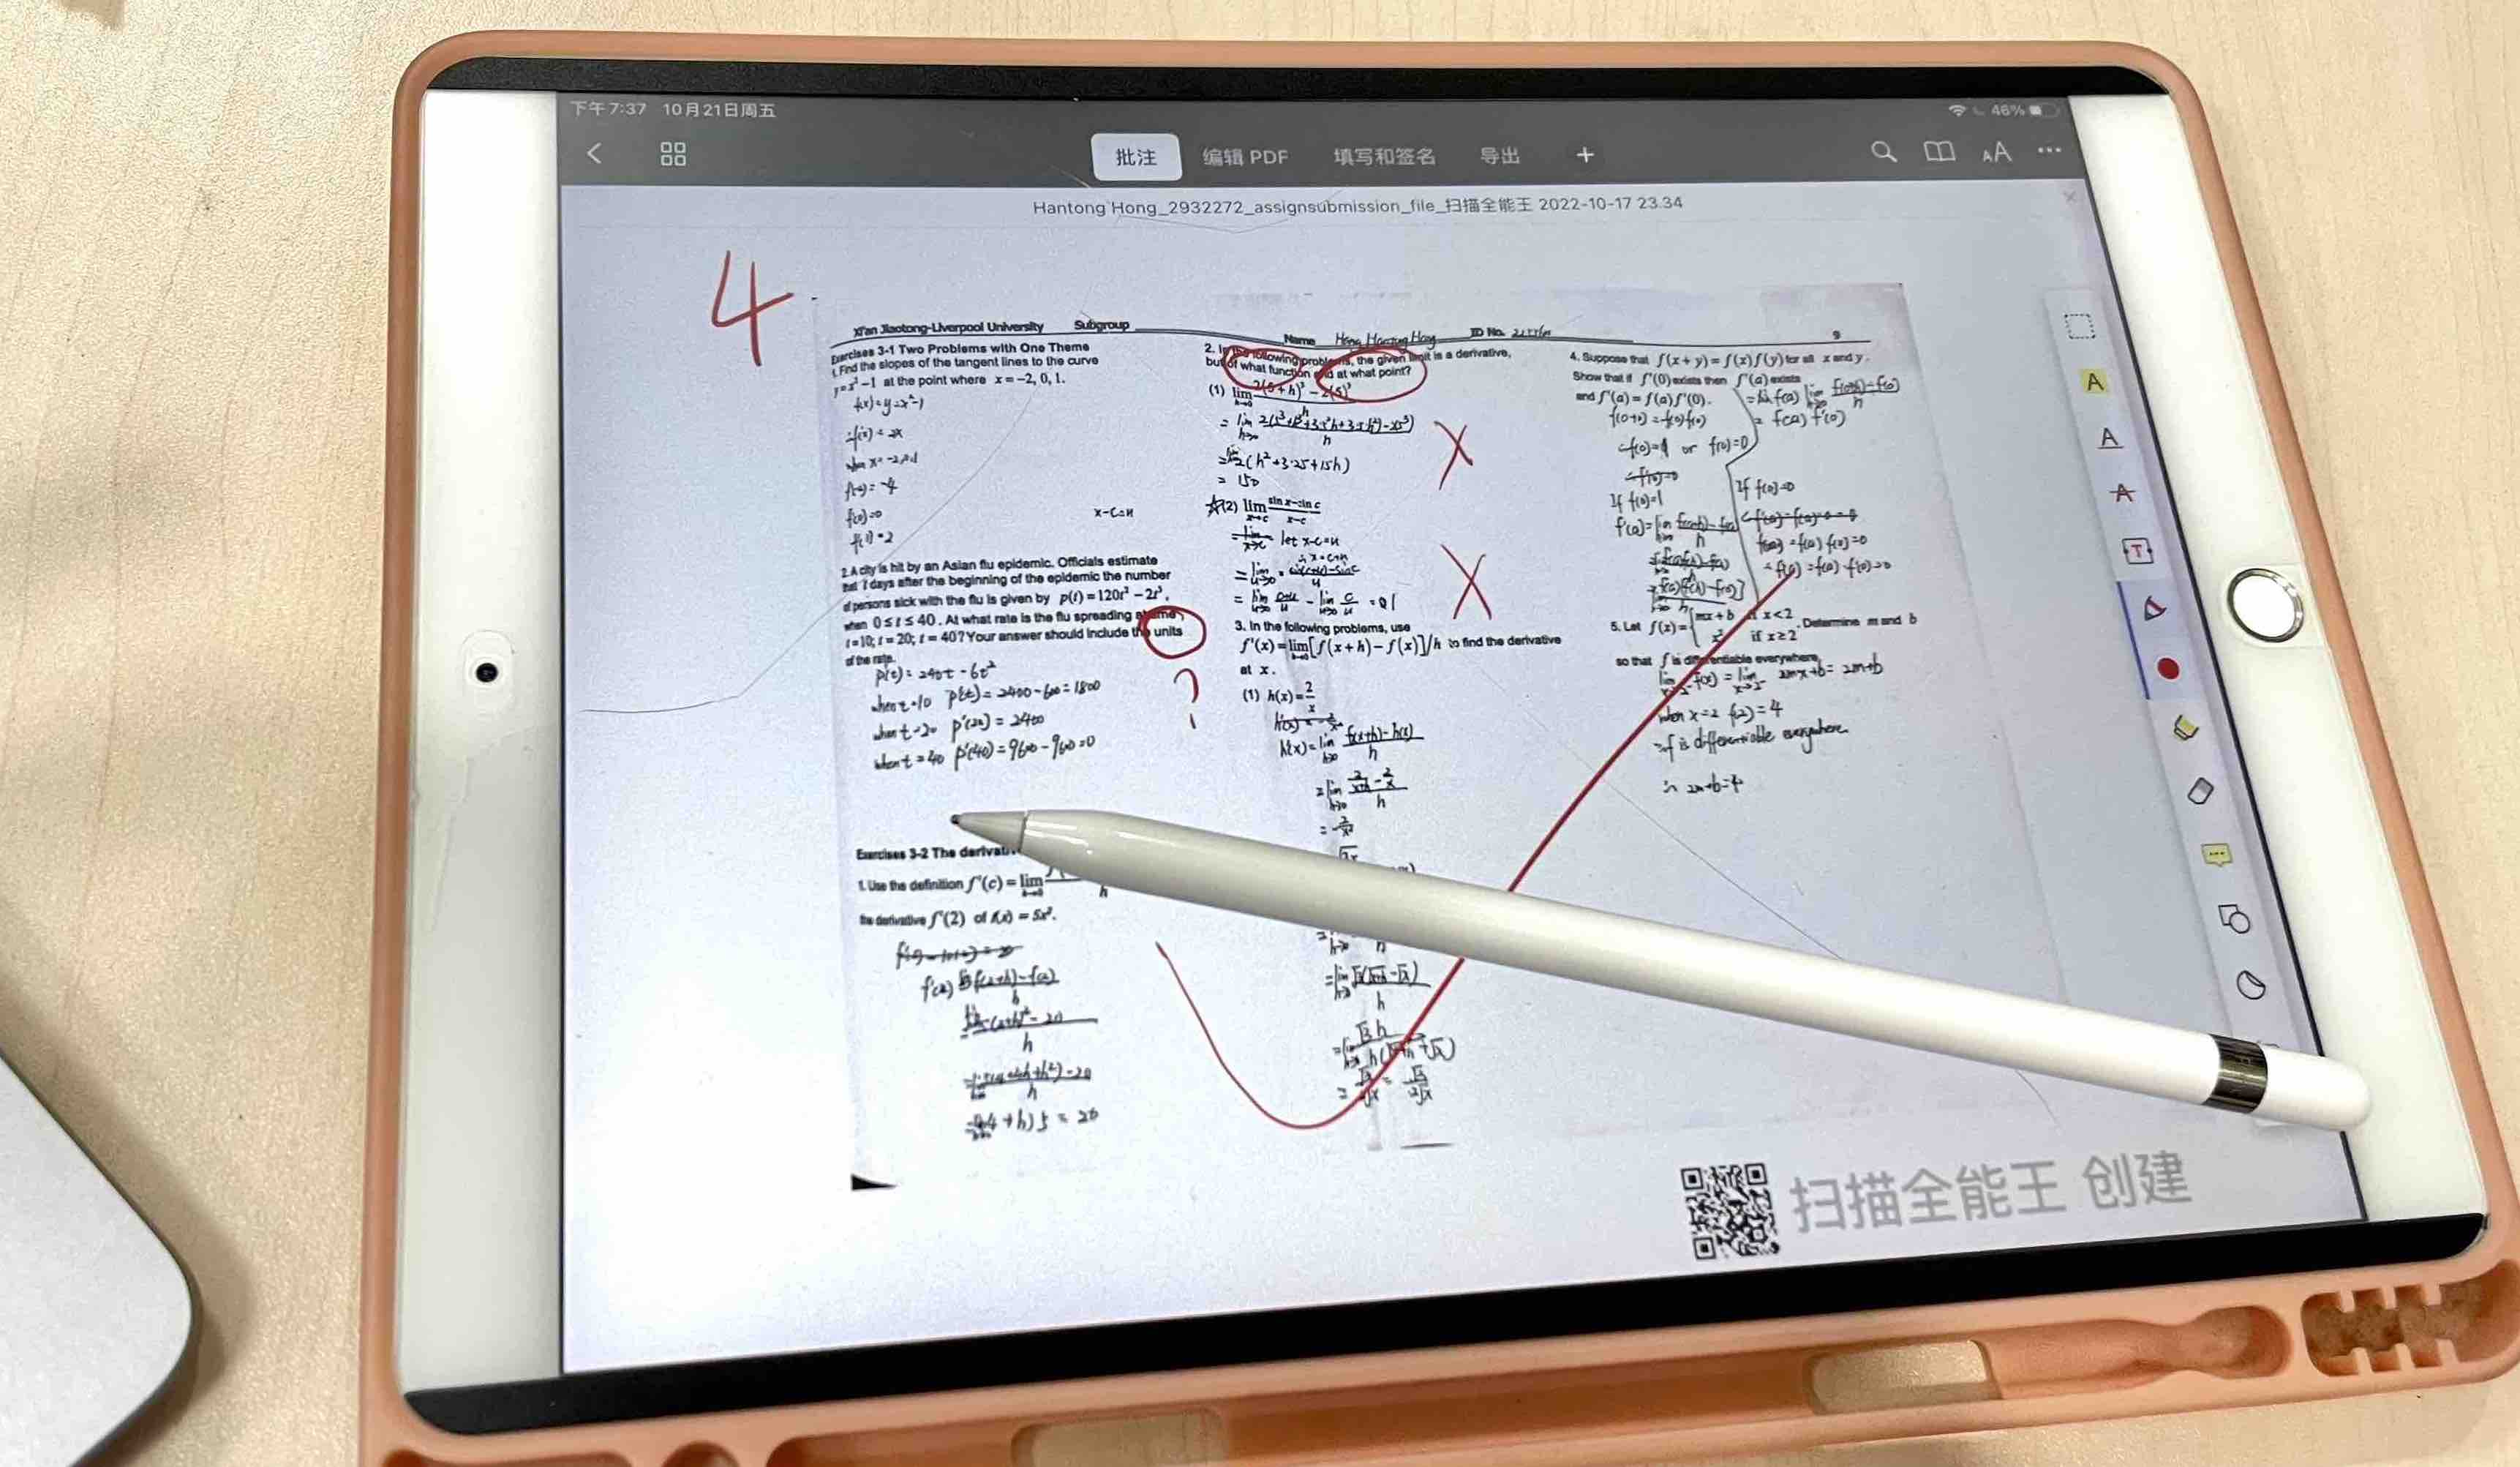
\includegraphics[width=0.5\columnwidth]{author-folder/Kai.Wu/marking_tools.jpg}
        \end{figure}
    \item 流水线提高效率:题多的时候,不要全部改完一个学生的作业再改下一份,这样尤其慢。尝试一下把作业分成几部分,先把所有作业的part 1(比如,前面三道题)改完,然后回过头来,改所有人的部分part 2(比如4-6题)。可能打开关闭文件会费一些时间,但这样能记住几个题的答案和评分点,改起来很快。切忌改每个作业都去看几眼答案。
    \item 同理,不要改完一个就登一个成绩。我的习惯是,把总成绩写一个巨大数字在左上角。全部改完过后,传电脑上,用最大号的缩略图(Mac:显示为图标,狂按command+等号;win:显示为超大图标),直接不打开文件就能看到左上角的分数。Excel里按姓名排序,文件夹里用名称排序,统起成绩来特别快。
        \begin{figure}[H]
            \centering
            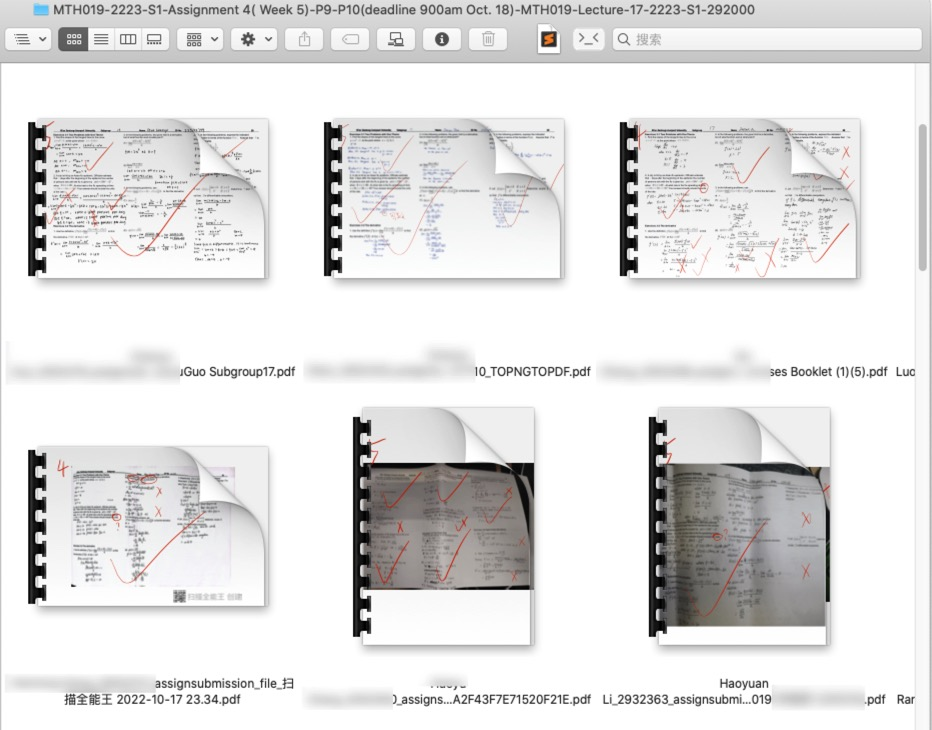
\includegraphics[width=0.7\columnwidth]{author-folder/Kai.Wu/tongchengji.jpg}
        \end{figure}
    \item 学生提交的文件可能有很多大病。比如,提交的不是pdf而是word甚至ppt、提交的pdf里面图片顺序是乱的、图片方向是错的、有标准的习题册不用而是自己拿个本写导致不好对答案。TA有权要求学生交作业的格式,可以对这些学生在feedback comments里面警告,并且提醒科任老师一定要在课上提醒学生,否则真的非常影响批阅效率。学生警告了仍然乱交格式时,可以按你的标准扣格式分。比如我的标准是:初犯警告,再犯扣20\%,三次扣50\%,四次扣完。
    \item 有时候文件巨大或者文件中有太多手写字迹,会导致pdf打开加载非常慢(一分钟甚至几分钟),而且容易崩溃。前者可以要求学生自行压缩PDF,后者实在是没办法。我写了一个Python程序\href{https://github.com/kaiwu-astro/xp_pgrs_unofficial_guide/tree/main/fileshare/pdf_to_png_to_pdf.py}{[GitHub链接]}应对这种情况,会在下载完所有作业过后把所有PDF转成图片再转回PDF,这样打开就不成问题了,文件大小也都能压缩到5M以内。需要的自取,但使用有点麻烦,不过我实在找不到其他更科学的方法了。
    \item (悄悄说)拿不准给多少分合适的时候,就给多一点。给少了,学生会找你argue,很浪费时间。给多一点,相当于节约自己的时间。
    \item 往表格登成绩的时候,难免犯错,登错或者登串成绩。初次或者前几次登成绩尤其容易出问题,可以考虑全部double check一遍。另外,如果你把成绩写在了PDF左上角,能一定程度解决这个问题,也就是如果成绩登错了,学生发现LMO成绩和PDF上的不一样,能马上联系你。
    \item 改完作业后,学生有可能会通过LMO给你发消息,或者给你发邮件。尽量不要直接回复学生,毕竟回复错了的话老师背锅。任何学生发给你的消息,请转给老师,让老师回复他。除非老师同意你直接回复。
\end{enumerate}

\begin{flushright}
    (2022年10月21日 by Kai Wu)
\end{flushright}

\subsubsection{批改试卷}
Quiz,期中,期末考试,助教有可能要参加评卷。所以期末放假跑路之前跟老师问清楚,以免要改期末卷但是不知道。如果确实有事要提前跑路,和老师商量。

\subsubsection{带Lab(实验课)}
\begin{newminipage}[0.55]
    像大学物理实验这种课,会让TA带实验课。物理实验的讲课流程一般是:先在实验室的白板给学生讲一下实验原理、数据如何记录和处理、注意事项,然后要亲手演示如何做实验。课后,要批改实验报告。

    我感觉,实验课非常有挑战性,因为确实就是实实在在的在大学里讲课。你需要自己花时间备课、准备讲稿、理清思路、准备学生可能问的各种问题;讲课前科任老师会对TA在实验室培训,你自己得先吃透如何做实验。还有突发事件如何处理,比如学生弄坏器材(及时问老师)。因为实验课就那么几节,总的工作时长加上批实验报告也比大部分其他课的批作业时长要少,但是非常锻炼人。可以挑战自己,如果不想干也一定要尽早跟老师、学院秘书提出换到其他课程。
    \begin{flushright}
        (2022年10月22日 by Kai Wu)
    \end{flushright}
\end{newminipage}
%
\begin{newminipage}[0.45]
    \begin{figure}[H]
        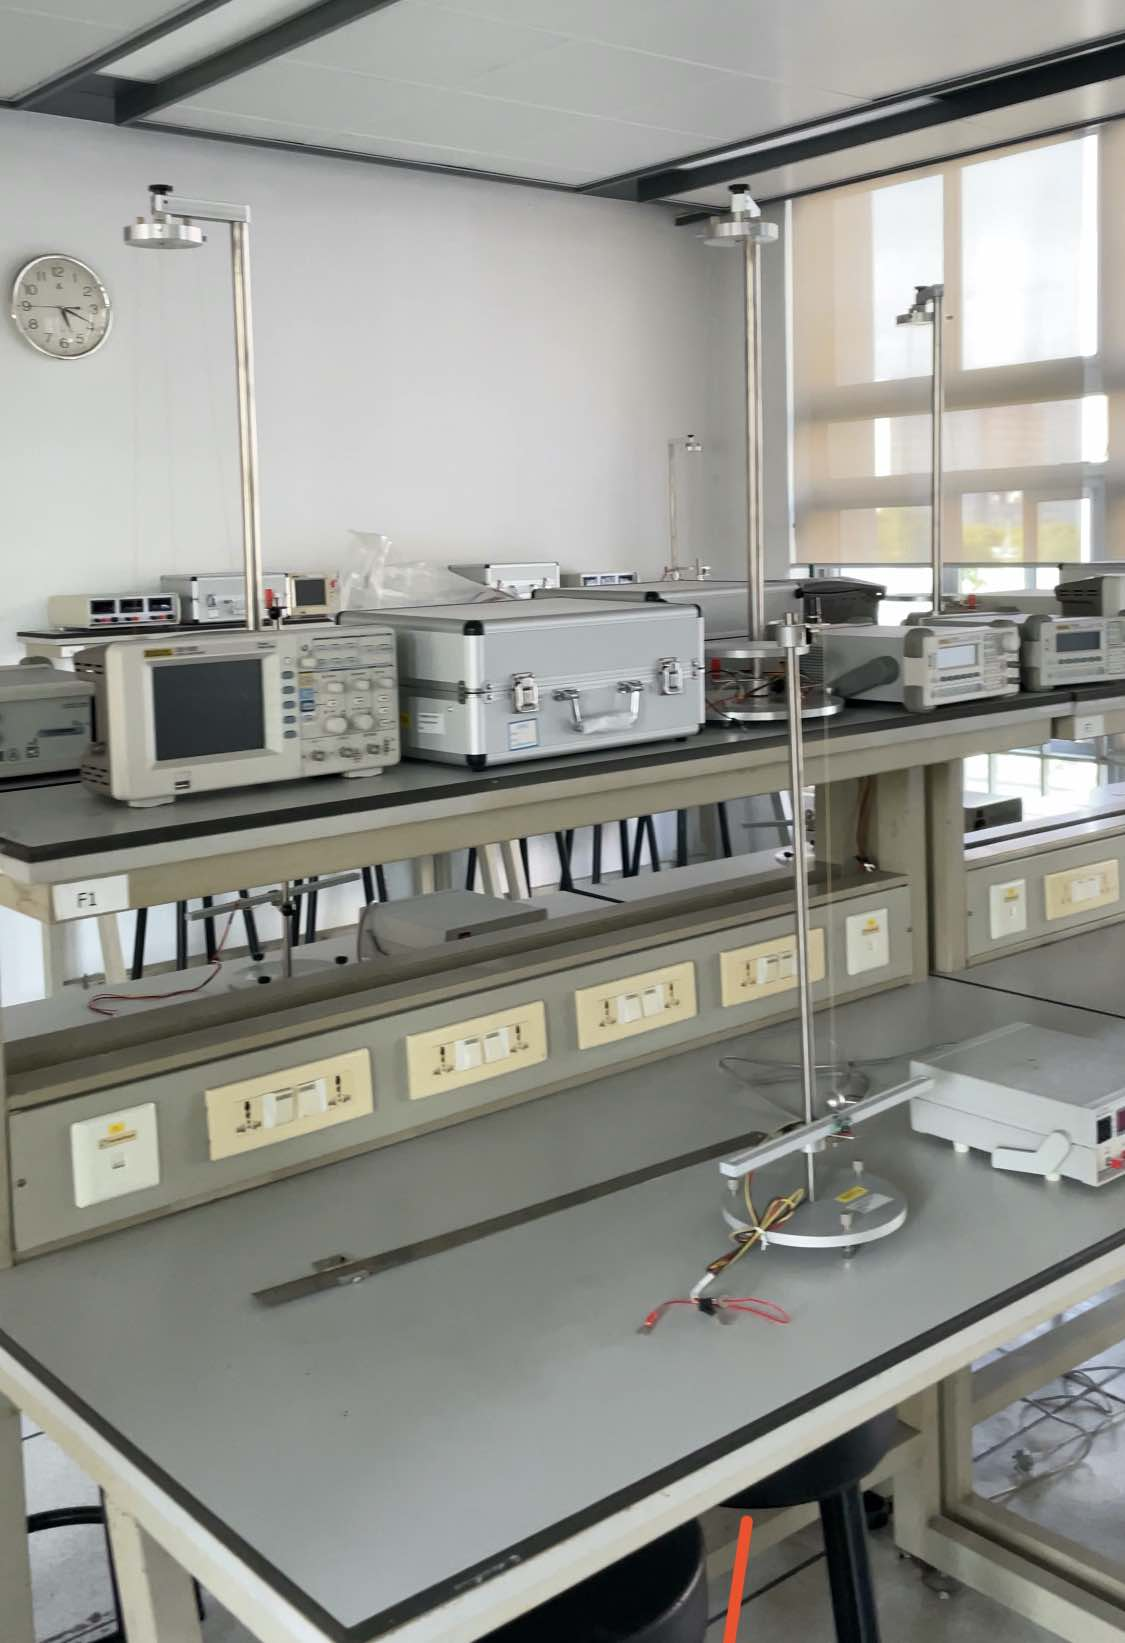
\includegraphics[width=0.95\columnwidth, right]{author-folder/Kai.Wu/lab.jpg}
    \end{figure}
\end{newminipage}



\subsubsection{如何做好讲Tutorial(习题课)}

\begin{enumerate}
    \item 课前做好充分准备工作,当你站上讲台那一刻,你就是一名教师了,要为自己说的所有的话负责,也要对学生负责。课前将课程所需要的材料拷到U盘中,进入教室后打开电脑登录自己的账号即可使用电脑。同时你也需要使用账号登录LM, AMS等乱起八糟的系统。由于学校电脑较卡顿,建议大家提前十分钟到达教室。此外,也需要提前十分钟下课,否则会被后面上课的老师和学生投诉你拖堂。
    \item 课后耐心回复学生的邮件与提问。此处给大家一个忠告,不要加轻易加学生微信,让他们有事有问题跟你邮件联系。否则你会变成一个7*24客服。邮件作为学校官方交流方式,很好的保护了教师和助教的私人空间和权益。曾经有学生投诉,就因为助教没有回复学生的微信。
    \item 有问题及时跟module leader沟通,遇到棘手的问题,不要自作主张,需要与module leader商量。学生给的反馈,也可以与co-teacher沟通,以提升学生的学习体验。学生体验感好了Module Questionnaire(MQ)分数自然就上去了。MQ的分数即学生评教分数,如果分数好看,求职的时候,是可以放到简历里的。
\end{enumerate}

\begin{flushright}
    (2022年12月30日 by Yue Zhou)
\end{flushright}

\subsection{TA工资是多少,怎么结}
2022年TA工资是60元/小时,每月一结,次月月底发钱。例如,2月底发1月工作的工资。

\emptyline{}
另外,期中、期末考试的监考也是TA的一种,会计入奖学金学生的TA工时,对自费同学,监考的工资单价一般也高得多。监考见下一节。
 \clearpage

\section{监考怎么做(挖坑待补)}

监考的工资单价一般比其他TA工作要高,2020年左右一般是100一个小时,而且准备工作比较少,监考途中基本也就是走一走,很轻松,是不错的挣钱方法。

\subsection{如何参加}
(我还真不知道最近怎么参加,之前我都是学校给分配的。谁知道来介绍下?)

\subsection{具体怎么做}
首先学校有监考的培训,在\textit{Teaching Assistant (TA) Training Programme}为题的邮件里的Assessment and invigilation那一项就是,或者是在你的LMO里翻一下。

(挖坑待填,如果没人需要,或者学校已经不用本校生监考的话那就不写了)

\begin{figure}[H]
    \centering
    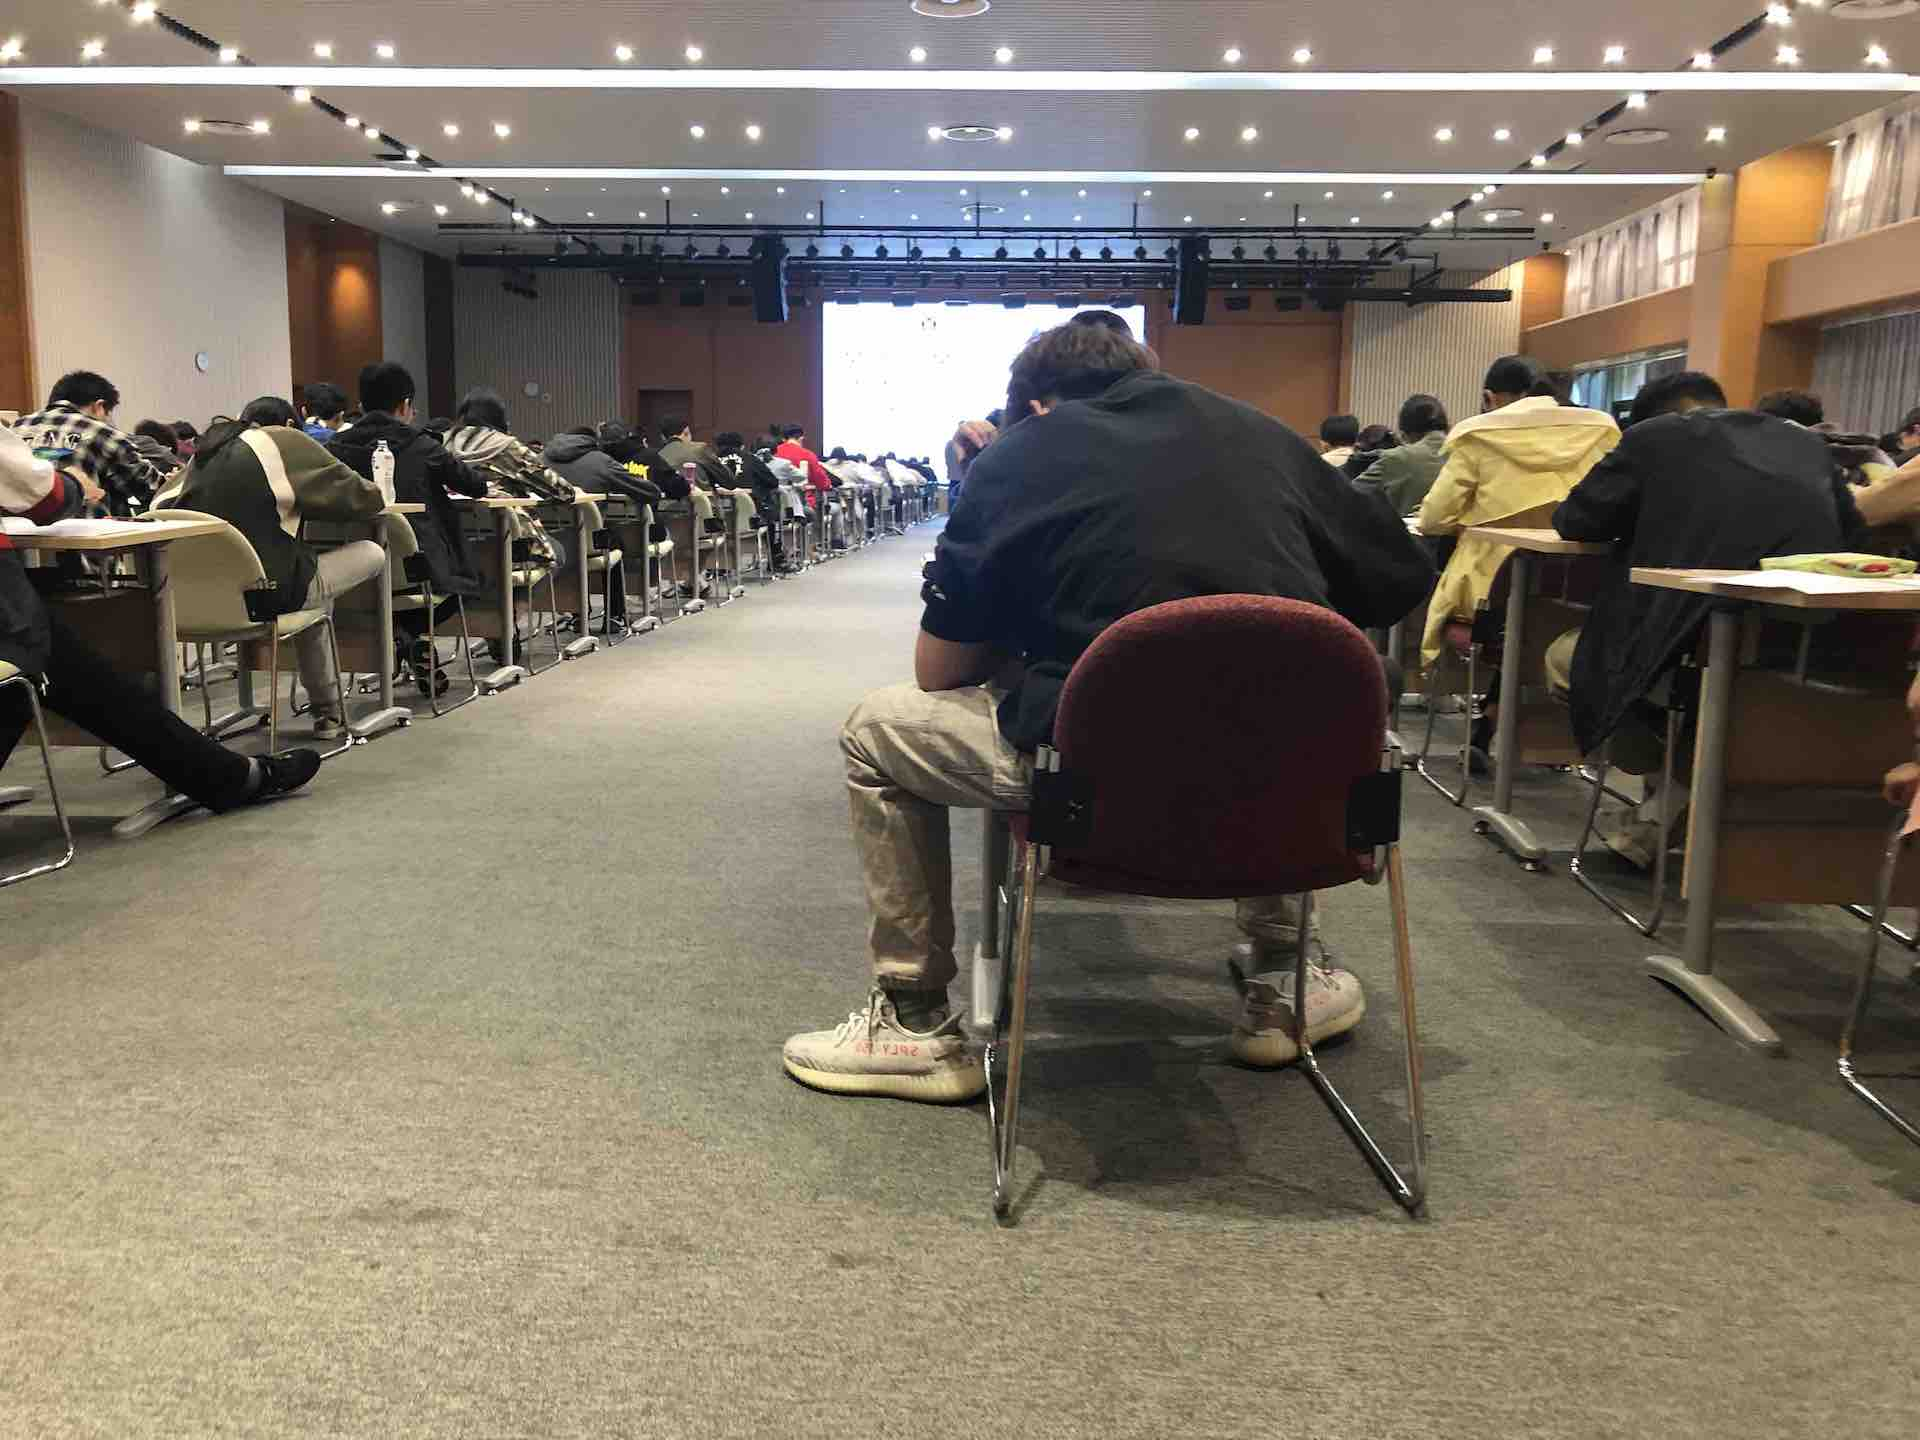
\includegraphics[width=\columnwidth]{author-folder/Kai.Wu/invigilation.jpg}
    \caption{2020年11月15日,CB楼G层某考场,监考中}
\end{figure}

\begin{flushright}
(2022年10月22日 by Kai Wu)
\end{flushright}

% \begin{figure}[H]
%     \centering
%     \includegraphics[width=0.5\columnwidth]{author-folder/Kai.Wu/}
% \end{figure}


% \usepackage[export]{adjustbox}

% \item 
% \begin{minipage}{0.3\textwidth}
%     文字
% \end{minipage}
% \begin{minipage}{0.63\textwidth}
%     \begin{figure}[H]
%         \includegraphics[width=0.4\columnwidth, right]{author-folder/Kai.Wu/}
%     \end{figure}
% \end{minipage}

% \input{author-folder/Kai.Wu/.tex}
 \clearpage

\section{和就业有关的重要信息(挖坑待补)}

关于学籍、学历、就业材料等,首先建议到学校就业中心阅读FAQ:\url{https://careers.xjtlu.edu.cn/Dispatch/Home/Master}

上面网站可能没涉及,或者问得很多的问题如下

\subsection{学籍·学信网?}

学信网查不到,去中外合作办学网站查

毕业证图片

\subsection{成绩单?}

liverpool life



% \begin{flushright}
% ( by Kai Wu)
% \end{flushright}

% \begin{figure}[H]
%     \centering
%     \includegraphics[width=0.5\columnwidth]{author-folder/Kai.Wu/}
% \end{figure}


% \usepackage[export]{adjustbox}

% \item 
% \begin{minipage}{0.3\textwidth}
%     文字
% \end{minipage}
% \begin{minipage}{0.63\textwidth}
%     \begin{figure}[H]
%         \includegraphics[width=0.95\columnwidth, right]{author-folder/Kai.Wu/}
%     \end{figure}
% \end{minipage}

% \input{author-folder/Kai.Wu/.tex}






%# -*- coding: utf-8-unix -*-
%%==================================================

\chapter{其他攻略}

\begin{flushright}
    ——看一眼不亏,看两眼血赚
\end{flushright}

\section{大坑:假如明天你突然丢失电脑所有数据怎么办?——如何备份资料}

\begin{figure}[H]
    \begin{tabular}{rl}
        
\includegraphics[width=0.5\columnwidth]{author-folder/Kai.Wu/backup1.png} &
        
\includegraphics[width=0.4\columnwidth]{author-folder/Kai.Wu/backup2.png}
    \end{tabular}
    \caption{\href{https://baijiahao.baidu.com/s?id=1719578217211021768}{链接:贵阳一女大学生8000字毕业论文保存失败崩溃大哭}}
\end{figure}

绝大部分同学本科就买了自己的电脑。虽然自己的各种作业资料,到现在博士阶段的研究数据、论文,全部就只存放在这一台电脑里,但并没有足够意识到自己电脑的重要,和保存在电脑里信息的脆弱。每年,都会有如上图的事情发生,给当事人带来上新闻被全国人民笑话的沉重打击。

丢失一篇正在写的论文,其实是小事,毕竟研究资料全部都在。上面新闻的当事人,其实也就用了几天时间就重新写好了论文。但那些万年不动、又极其重要的资料,又是绝对安全的吗?

想象一下,假如
\begin{itemize}
    \item 你某天手一滑,电脑摔倒地上,再也开不了机,硬盘也没法恢复
    \item 头昏脑涨的一天,你接了一杯咖啡,一不注意,咖啡撒在了电脑上,瞬间短路,电脑滋滋冒油
    \item 你不慎点击了一个链接,中了勒索病毒;或者,西浦内网被网络攻击攻陷,所有电脑中勒索病毒。你的所有文件被加密封锁。
    \item 你把电脑带出去办公或者采集数据,整个电脑直接被偷走
    \item 你过年回家,在路上,背包或者行李箱被人偷走了或者拿错了
    \item 无恶意,但万一,西浦着火了,西浦进水了(MB的5楼一下大雨就漏水),西浦楼塌了,撤离的时候你根本来不及拿电脑
\end{itemize}


\begin{figure}[H]
    \centering
    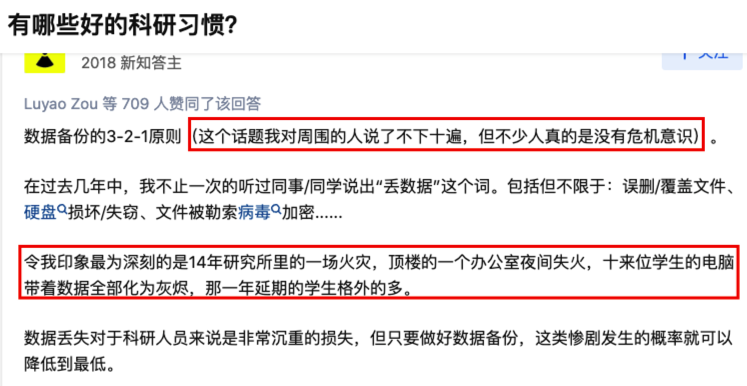
\includegraphics[width=0.8\columnwidth]{author-folder/Kai.Wu/backup_zhihu.png}
    \caption{\url{https://www.zhihu.com/question/394796969/answer/1501840215}}
\end{figure}

这些情况,单个可能很罕见,但所有可能性加起来,再乘以3到4年时间,至少发生一次的概率并不小。如果发生,你的博士进度会被耽误多久,你的青春又会被耽误多久呢。

只有一份的数据是非常脆弱的。现在思考一下,你赖以生存的电脑、数据、论文,是否只存了一份?如果是,请立即把屁股从椅子上挪起来,去厕所洗把脸,问问自己都是成年人了,怎么心这么大,然后开始看下面的攻略。

\subsection{理论:321原则}

「3-2-1 原则」是商业公司通用的数据备份金方法,具体内容是:
\begin{itemize}
    \item 3:存储 3 份完整文件,一份原件加上两份拷贝。
    \item 2:将文件起码保持在两种不同的介质上。
    \item 1:将一份拷贝保存在异地。
\end{itemize}

所谓的「介质」,是指内置硬盘、移动硬盘、U盘、网盘等不同的存储介质。说起来好像很麻烦,但对我们来说最简单的实践是:原件保存在内置硬盘,将两份拷贝分别存到移动硬盘和网盘,就同时达成了三条要求。这时,你回过头去看一下我上面列举的所有可能的灾难性问题(甚至即使是网盘公司突然倒闭),都能做到游刃有余,不影响你的科研!

\subsection{实践}

到动手准备的环节了。首先根据你手里的资源,决定你要备份的范围。最土豪的情况,你可以把整个电脑做一个本地备份 + 云端网盘备份,但很多时候,要么网盘容量很小,要么移动硬盘容量不够,要么网速太慢把太多资料传网上很慢,所以先划定你的备份范围。

\begin{itemize}
    \item 最经济的方案:只备份最重要的文件。例如:论文、科研资料、CV、电脑桌面,等等。网盘实时备份+移动硬盘定期备份。对移动硬盘和网盘容量要求都很小。
    \item 最高效的方案:整个电脑(包括最重要的数据)本地备份;最重要的科研、论文等加一分网盘实时备份。这需要一块比你电脑硬盘更大的移动硬盘(不贵),加正常容量(10个G左右)的网盘。
    \item \sout{最土豪的方案:买个NAS,插几十T的盘,组RAID1,再实时传一份到异地。}
\end{itemize}

正常电脑硬盘容量一般在2T内,另外我假设大家去买一块2T以上的移动硬盘(500块以内)应该压力不大(导师经费较多的,可以直接问导师要,直接说想要一块移动硬盘做备份问导师能不能帮忙买就行,2000块以内报销都很简单)。所以下面只介绍中间的高效的方法

\subsubsection{电脑整机备份}
\label{sec.pc_backup}

把电脑整机备份的一大好处就是,假设电脑直接灭失,新买一台电脑过后,能在一天之内完全恢复之前的工作状态,无缝衔接,科研毫不受影响。

Windows和macOS都自带系统级的整机备份方案。网上攻略特别多,我就不废话了。
\begin{itemize}
    \item Win请在b站直接搜索windows备份看教程,一般使用系统的“备份与还原(windows7)”(虽然名字里有win7但win10和win11也是完全能用的,这也就是为什么一直没被扔掉),比如看这个视频 \url{https://www.bilibili.com/video/BV1Dy4y1x7RP}
    \item macOS请在b站直接搜索mac time machine,一般使用系统设置里的“Time Machine”,比如看这个视频 \url{https://www.bilibili.com/video/BV1oy4y177qS}
\end{itemize}
一个视频看了不太明白没关系,多搜几个看,也同时善用谷歌、知乎等。初学者可能感觉学习成本有点高,但不要等到电脑炸了再开始准备呀。

\subsubsection{网盘备份}
\label{sec.net_drive_backup}

学校的box使用的是seafile网盘系统,今年升级到了每人100G的免费空间,内网备份速度超级快。把最重要的文件夹拖入seafile(不用移动文件夹),他就会自动实时备份到网上。使用方法见\url{https://guide.xjtlu.edu.cn/box/student/drive_client/drive_clent_for_windows.html}

另外,如果对学校IT不放心,可以同时安装一个另外的商业网盘进行第二重网盘备份。个人严重不推荐百度云,因为偶尔会随机吃文件。国内的,我个人推荐坚果云(免费版无限空间,但限制每月流量),国外网盘推荐Onedrive(个人版免费5G,可在淘宝搜索onedrive扩容花几块钱扩容到永久15G)。另外,大家的利物浦账号下都有免费1T的Onedrive,羊毛薅起来(但注意毕业前得把数据迁出去,因为毕业了要收回账号),参见这一章节 \ref{sec.fuli_liverpool}。


\subsection{论文备份·文件历史版本}
\begin{newminipage}[0.65]
    上述备份防灾的方法可以应对绝大多数数据丢失的场景。但,各位的论文,包括毕业论文和期刊发表的论文,作为最重要也是最脆弱的资料,除了怕丢失还特别怕这两件灭顶之灾:
    \begin{enumerate}
        \item 版本混乱。论文从一开始写到写完,中间修改个几十版是常事。特别是在临近提交的时候,一定会由于导师意见、二导意见、合作者意见等再battle个十几版出来。其中各版本的区别可能非常小,肉眼也很难分辨。一定会有一天,你也搞不清楚哪个是哪个版本、忘了在哪个版本作了什么修改,会在分辨版本上反复花费时间,进而导致 ↓
        \item 文件覆盖,例如(1)新版本直接覆盖了老版本,但过一段时间又因为某种原因要拿回老版本 (2)老版本覆盖了新版本,几个月的论文白改
    \end{enumerate}
\end{newminipage}
\begin{newminipage}[0.34]
    \begin{figure}[H]
        % \caption{导师:把最终版发给我}
        
\includegraphics[width=0.95\columnwidth, right]{author-folder/Kai.Wu/thesis_versions.jpg}
    \end{figure}
\end{newminipage}

读到这里,你如果感兴趣可以做个实验,创建一个文件,里面写上一些内容。然后在其他文件夹新建一个同名文件,写上另一些内容。最后,把它拖过来,覆盖掉前面的文件,这时,试一试自己有没有任何办法找回前面文件的内容。

你可能要问,上面不是说了这么多备份方法吗?是的,这些备份方法主要的作用是防丢失,比如电脑丢失、硬盘损坏,但少有备份能做到防覆盖。比如,实时备份的网盘,你本地把文件错误覆盖了,云端也马上被覆盖了。本地备份硬盘,如果备份频率不高,则还有一线生机,但如果过一段时间再去找,也可能找不到了。

因此,为了你的论文(命根子)安全,完全值得再加一层保险:

\begin{enumerate}
    \item Windows开启系统级的文件历史保护:\url{https://www.asus.com.cn/support/FAQ/1013067/},别忘了一定要把你的论文文件夹添加进去才能生效
    \item mac的TimeMachine(时间机器)备份自带了文件历史功能。参照前面的 \ref{sec.pc_backup} 配置好TM,整个电脑的文件历史就都包括在备份里了。
    \item Linux用户,我相信你们有的是办法。最笨的办法,直接写一个shell脚本,把论文文件夹直接复制到其他目录、用日期命名,最后把这个脚本加到crontab里定期运行即可。
    \item 以上是开启本地文件历史的方法。一些网盘自带文件版本功能,但一般限制版本数量或者日期,或者必须要买会员才能开启文件版本。开启过后,相当于云端也存了一份版本历史,万一本地的你没设置好或者其他什么原因不能用,还能在错误覆盖的时候救你一命。学校的seadrive自带大概两个月的文件版本,免费,非常良心,再次建议大家使用。直接把文件夹拖进去备份,就会自动产生文件版本。参见章节 \ref{sec.net_drive_backup} 。
    \item 会一点Git、GitHub的同学,请直接把整个论文文件夹创建成Git项目,并上传到GitHub做成private repo,每天工作结束后交一个commit来备份版本,同时记录你修改了什么内容。对于论文,Git是最完美的备份方案,可以轻松回滚到老版本同时从不担心覆盖、甚至能轻松知道哪个地方的修改是在什么时候引入的,比以上所有方法都靠谱。Overleaf也有GitHub集成,可以方便的与导师协作。但Git学习成本略高,不过网上有无数详尽的教程,感兴趣、学有余力的同学可自行学习。
\end{enumerate}


\begin{flushright}
(2022年12月02日 by Kai Wu)

(major update: 2022年12月30日 by Kai Wu)
\end{flushright}

% \begin{figure}[H]
%     \centering
%     \includegraphics[width=0.5\columnwidth]{author-folder/Kai.Wu/}
% \end{figure}


% \usepackage[export]{adjustbox}

% \item 
% \begin{minipage}{0.3\textwidth}
%     文字
% \end{minipage}
% \begin{minipage}{0.63\textwidth}
%     \begin{figure}[H]
%         \includegraphics[width=0.95\columnwidth, right]{author-folder/Kai.Wu/}
%     \end{figure}
% \end{minipage}

% \input{author-folder/Kai.Wu/.tex}
 \clearpage

\section{远程控制·如何校外访问校内电脑}

人在校外的时候,经常会很想念校内的电脑。不管是学校给大家每人配的小台式,还是用导师经费买的的其他电脑,都可以远程控制。

\subsection{学校配的电脑·准备工作}
(如果不是想访问学校配的电脑请直接跳到下一节)

学校给的电脑比较特殊,默认我们不能安装软件。有两种办法
\begin{enumerate}
    \item 发邮件或者打电话给IT,直接问他们要管理员权限。就说你是博士生,要在学校给的电脑上装软件。之后就可以装控制软件了
    \item 上面这种办法过后,电脑还是归学校管理,仍然有一些限制,但对普通使用基本够了。\sout{(有强迫症)}想完全控制学校电脑的同学\sout{(比如我)},可以直接格盘重装系统,或者分区(保留原系统)另装系统做双系统。windows重装系统、分区做双系统的教程,b站和知乎特别多。
\end{enumerate}

\subsection{桌面控制软件推荐}
以下软件不分系统,win/linux/mac均可用。
\begin{itemize}
    \item VNC: 被控端(学校电脑)安装 VNC Server \url{https://www.realvnc.com/en/connect/download/vnc/},控制端(你手上的电脑)安装 VNC Viewer \url{https://www.realvnc.com/en/connect/download/viewer/},注册账号登录使用,无需记录连接码。推荐理由:VNC是饱经检验的远程桌面,只要网络不挂,一般不会有问题。
    \item ToDesk:\url{https://www.todesk.com/}两边电脑软件一样。推荐理由:新兴软件,流畅度一般比vnc好一些。
    \item 其他:anydesk,Teamviewer,向日葵,均可尝试。其中,不太推荐Teamviewer,虽然老牌,但因为很可能检测到西浦的网络环境过后强制购买商业版,其他软件无此问题。
\end{itemize}

\subsection{远程SSH}
(不用linux的同学可直接跳到下一节看踩坑)

如果被控端是linux,你又主要使用命令行操作,那在桌面控制外,直接设法连接SSH,速度会快特别多。

电脑在学校是10开头的内网ip,如何在外面SSH?这种奇技淫巧叫做【内网穿透】

首先推荐这个视频:

\href{https://www.bilibili.com/video/BV1Qq4y1w7F5}{【硬核】公网访问?内网穿透!零经验上手!}\url{https://www.bilibili.com/video/BV1Qq4y1w7F5}

视频里校内机器可用的方案有两个,分别是

\begin{itemize}
    \item 视频的04:52,用IPV6连接。但要注意,我实测学校IPV6不稳定,过几天就会出现有v6地址但不能上v6网站的情况,更别提访问。即使你能做ddns,我个人也不推荐。
    \item 更靠谱的是视频08:09介绍的大内网穿透。免费易用的方案有:Zerotier(在境外,略慢),花生壳(国内老牌,但注册需要身份证),NOFRP(新兴,可靠性可能不高),或者直接在b站搜【免费内网穿透】,会有很多新方案。这几个方案如果不太会,b站、知乎有大量教程。
    \item (进阶大流量版,但学习成本较高)免费的方案对流量和带宽的限制都比较大,只是SSH执行命令完全足够了。但如果你想要奢侈的用scp拷文件,或者用SSH转发VNC,请考虑用导师的钱租一台云服务器,手动搭建frp服务(比较麻烦,但操作完过后用起来很爽,转发VNC比前面几种远程桌面都快),甚至,在宿舍宽带下弄个垃圾机器做跳板机,搞到公网ip,配合ddns,无限流量访问。这些方案学习成本较高,有兴趣的可以参考网上教程慢慢折腾。
\end{itemize}

\subsection{踩过的坑}
下面是我踩过大量坑过后从坑里带出来的经验:
\begin{enumerate}
    \item 冗余提高可靠性:不要只用一个远程控制方案,万一挂了一个,还能用另一个。请至少安装两个,如果是长时间不在校,可以安装更多个。我自己用的是:家宽里用一台二手瘦主机搭frp加ddns + 花生壳作backup-plan + vnc作another-backup-plan + ToDesk四重备份方案,稳定访问校内的linux电脑。
    \item 安装完成后,重启一次,看下控制软件是否能自己启动。
    \item 如果被控端是windows电脑,请务必屏蔽系统更新。虽然重启没问题,但windows大版本更新过后,会卡在一个让你同意新的用户协议的界面,除非你到场点一下,所有软件都不会启动,也就直接失去控制。请百度【禁止windows更新】。个人建议用组策略+改host组合拳。
    \item 跑程序的同学,请务必注意,不要超内存,不要炸系统内存。内存一吃满,系统立即死机,控制软件全杀完,而且还不会自己重启,必须要到场强制重启。请一定想办法在程序里监测、控制内存用量。
    \item 有条件的可以购买【向日葵控控】这样的远程KVM硬件,即使死机也可以自己远程强制重启。
    \item 再好的方案,也敌不过学校网络维护断网和学校施工断电。而这些,也是可以防御的。应对断网,请注意在网络登录时勾选macauth,网络维护完了就又能用了。来电自动启动功能,需要主板支持,在主板说明书搜索boot on power或boot with power,或直接搜power,看看有没有。或者,购买向日葵控控。不过断电断网始终是极少数时候,除非你一走几个月,基本不需要考虑\sout{(但万一被隔离了呢)}。
    \item 请和至少一个在校同学搞好关系,新手总会遇到各种意外的情况失去控制,需要办公室同学帮你跑腿看机器情况。100种远程控制的方案背后,也需要好同学做物理控制。万一的万一,哪天网线被人不小心踢掉了呢,还是只有\sout{通过py交易}让同学帮你弄。
\end{enumerate}

\begin{flushright}
(2022年11月09日 by Kai Wu)
\end{flushright}

% \begin{figure}[H]
%     \centering
%     \includegraphics[width=0.5\columnwidth]{author-folder/Kai.Wu/}
% \end{figure}


% \usepackage[export]{adjustbox}

% \item 
% \begin{minipage}{0.3\textwidth}
%     文字
% \end{minipage}
% \begin{minipage}{0.63\textwidth}
%     \begin{figure}[H]
%         \includegraphics[width=0.95\columnwidth, right]{author-folder/Kai.Wu/}
%     \end{figure}
% \end{minipage}

% \input{author-folder/Kai.Wu/.tex}
 \clearpage

\section{我的老腰受不了了——如何保持颈椎、腰椎健康}

\subsection{缓解腰的问题:升降桌}

\begin{newminipage}[0.39]
    \begin{figure}[H]
        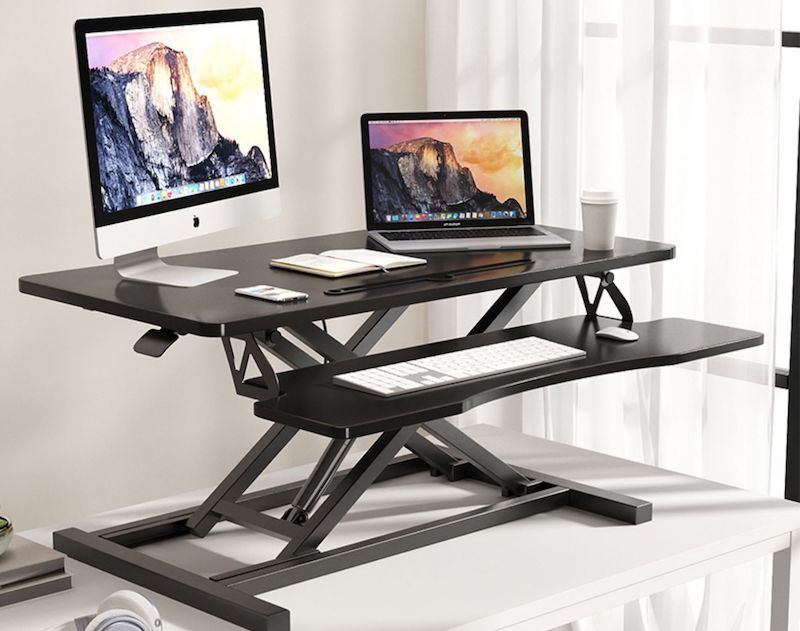
\includegraphics[width=0.95\columnwidth, right]{author-folder/Yue.Zhou/gongzuotai.jpg}
    \end{figure}
\end{newminipage}
\begin{newminipage}[0.6]
    在没有读博之前,我就患上了严重的腰肌劳损。这个玩意怎么说呢,说是大病吧,他不是,但无时无刻不在折磨着你。最严重的时候,疼的我晚上都睡不着。去医院看过也开过药,但医生说这个病需要自己保养,无法根治。后来我试着跑了半年步,哎!腰肌劳损神奇的好了,现在一点都不疼了(如遇久坐,仍旧是不行的,会疼)。读博之后也没有心情运动了,于是买了一个升降工作台(推荐人手一个!太好用了!)。可以站着办公,站累了就坐下办公。极大程度上杜绝了久坐对腰椎的伤害。
\end{newminipage}

\begin{flushright}
(2022年12月30日 by Yue Zhou)
\end{flushright}

\subsection{来自重度腰椎间盘突出、颈椎病患者的深度建议}

\subsubsection{升降桌:可极大缓解腰椎问题,但不能完全解决}

我十年腰椎间盘突出加五年颈椎病,19年的时候腰就疼到没法坐一整天,就在实验室放了台升降桌,站着用了三年电脑。今年还在卧室里放了同款升降桌。但长期站着和坐着一样对腰不好,最后会变成站着和坐着一样会腰疼。升降桌不是长久之计,站着只是换了角度继续损耗腰椎。

不能完全依赖升降桌:这几年太依赖升降桌,导致现在长时间站着和坐着一样腰疼,去拍核磁医生都问我是不是腰骨折了。如果真的想缓解腰疼,就要避免久坐久站。中学教师容易得腰疼一方面就是因为站着讲课时间长了。

总之升降桌可以用,但不能长期用它代替坐着用电脑。可以交替用,平时再多锻炼就行。

注意事项:升降桌记得没事调一调高度。我放实验室里的升降桌几年没调好像液压杆生锈了,都调不动了,直接变成了一般桌子。

\subsubsection{外接屏:避免和缓解颈椎病}

颈椎病难受的一点就是,低头时间长就脖子疼,出门在地铁高铁上我都不得不把手机竖起来抬高和眼平行,不然用不了太长时间。

我再贡献一个避免和缓解颈椎病的方法,就是不要长时间用笔记本电脑,长时间低头看屏幕会演变成颈椎病。低头看手机也是。

如果常用笔记本电脑就要在卧室和办公室都放一个台式机屏幕当外接屏。

我颈椎病就是高强度用了一年笔记本电脑得上的,后来只用外接屏就不再继续加重了。

如果经常高强度用笔记本电脑,不用外接屏的话和整天低头用手机一样都是颈椎杀手。我在实验室看见有人长时间用笔记本都会劝他们用外接屏。

笔记本支架也可以,比显示器便宜。但如果视力不好,还是尽量外接屏,因为笔记本屏幕太小了,费眼。我以前也买了很多笔记本支架,现在都用来放显示器了,笔记本刚好能放在下面很方便。

\begin{figure}[H]
    \caption{我自己在卧室里就是升降桌,配笔记本支架。这个组合很适合我这种主要用笔记本的}
    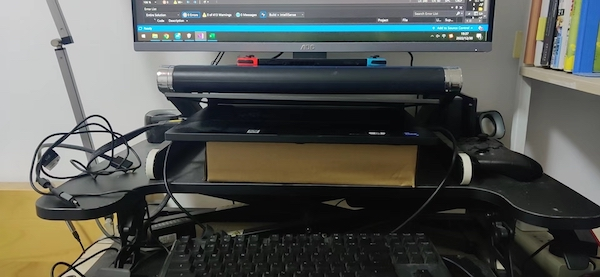
\includegraphics[width=0.95\columnwidth, center]{author-folder/Jialin.Wang/shengjiangzhuo.jpeg}
\end{figure}


% \subsubsection{进一步缓解:趴着用电脑}

% 我今年起站也不能站太长时间,已经开始探索平躺和俯卧用电脑了。平躺我试过几天就放弃了,容易睡着。我觉得平躺就适合看看电影玩游戏。

% 俯卧我最近试了一个月,感觉还行,起码支起上半身不会犯困。

% 我是放了一个便携屏幕在床边,然后配一个趴枕,这样能趴一整天。趴枕好处是吃完饭趴着不会压迫腹部导致不适。

% \begin{figure}[H]
%     % \centering
%     
\includegraphics[width=0.3\columnwidth, center]{author-folder/Jialin.Wang/pazhen.jpeg}
% \end{figure}

% 然后配一个可以调角度的笔记本支架放屏幕键盘和鼠标——其实直接放笔记本也行,但发热量大,搬来搬去不方便。用便携屏能快速在升降桌和俯卧之间切换——我也想过买一般的显示器支架,但没有卖那种适合在床上用的,而且一般显示器在床上用太大了。便携屏就是笔记本二手屏幕改装的,大小和笔记本电脑一样在床上用正好。

% 如果长时间趴着用电脑,我发现最好是用双臂稍微用力撑起上半身。但上半身主要还是靠着躯干受力,双臂是辅助作用,避免下巴受力太大。

% 我现在已经练成了能俯卧一天的神功,笔记本支架只要调好角度,让手和手臂平行,这样手腕就不会因为长时间弯曲而酸痛。

% 不过最近因为趴习惯了加上天冷就完全不锻炼,如果不趴着,还是腰疼。还是得坚持锻炼才行。

% 这一套方案我觉得真的完美适合我这种腰疼到无法长时间坐着和站着的人,但这些都不能治好腰疼。锻炼才是最重要的。时间长不锻炼,不常用的肌肉会萎缩,更不好。(我好想以后住在热带沿海地区,每天傍晚去海边游泳,傍晚的时候海水是温的)


\subsubsection{最好的解决方案:改变生活习惯、加强锻炼}

建议有腰椎间盘突出和颈椎病的人还是多锻炼。但不要盲目去健身房锻炼,最好的锻炼方法还是游泳,因为其他锻炼方式大多会需要腰部用力,加重腰疼。

我目前只是偶尔腰疼到不能弯腰。我还认识腰疼到走路一瘸一拐的,他也是慢慢锻炼才逐渐好转。

如果自制力不强,加学校游泳社团也行,起码有人经常一起去锻炼能有动力。

办卡的话,我记得每年九月份独墅湖游泳馆能办半价年卡,但学校社团很便宜,更划算。以前我办游泳卡前每周都跟着学校游泳社团去游一两次,办了年卡后,一年去了不到五次,后来就去得更少了。
如果自制力可以,每天锻炼是最好的方法。
如果坚持不下去,还无法改变生活习惯,就会越来越严重。

最后,如果腰疼比较严重,有空可以去医院骨科看看,做一下核磁,看一下腰椎到底发展到哪个地步,来决定怎么具体该恢复。现在腰疼在年轻人里很普及。

\begin{flushright}
(2022年12月30日 by Jialin Wang)
\end{flushright} \clearpage

\section{西浦虚拟机}
\url{https://vdi.xjtlu.edu.cn/portal/webclient/index.html}
如果在学校外面,想临时快速访问学校内的资源、软件,可以使用学校的在线虚拟机。虚拟机相当于放在校内的一台电脑

\section{图书馆的文献数据库}
连接校园网后,绝大部分学校订阅了的期刊论文都可以直接在论文页面下载,但(1)有的期刊官网不能识别你的IP,甚至例如著名的Annual Review系列 (2)如果你在校外也想下论文,这时就可以用到图书馆的论文数据库

\begin{figure}[H]
    \includegraphics[width=0.7\columnwidth, center]{author-folder/Kai.Wu/library-ejournal.jpg}
\end{figure}

我用得最多的是在首页 \url{https://lib.xjtlu.edu.cn} 点击e-journal,按期刊名称搜索期刊,然后就可以跳转专有链接访问。同时,图书馆还提供了很多全文数据库,甚至还有知网等中文期刊数据库。详细的使用姿势,见图书馆往期培训 \url{https://core.xjtlu.edu.cn/course/view.php?id=905} ,或者直接本项目的GitHub里(\href{https://github.com/kaiwu-astro/xp_pgrs_unofficial_guide/tree/main/fileshare}{链接})找到PPT。

\section{苏州图书馆借书和免费送书}
想看独墅湖图书馆的书,想借苏州图书馆的书,但是太远了不想去怎么办?直接小程序借书!苏州图书馆的书可以\textbf{【免费】}送到独墅湖图书馆取书,而独墅湖图书馆的书可以直接送到学校图书馆门口。
微信搜索【苏图借书】小程序。因为医保卡就是市民卡可以直接拿去借书,如果你已经拿到了医保卡,可以直接绑定医保卡,免开卡费。然后在小程序内按提示操作即可。
% \section{学生医保}
\section{重视自己的负面情绪和抑郁倾向}
\label{sec.mental_health}

\begin{figure}[H]
    \includegraphics[width=0.6\columnwidth, center]{author-folder/Kai.Wu/mental_1.pdf}
    \includegraphics[width=0.6\columnwidth, center]{author-folder/Kai.Wu/mental_2.pdf}
    \includegraphics[width=0.6\columnwidth, center]{author-folder/Kai.Wu/mental_3.pdf}
\end{figure}

伯克利研究生会2014年发表的\href{http://ga.berkeley.edu/wellbeingreport}{研究生幸福和健康报告[链接]}显示,46\%的博士生存在心理健康问题。Nature等权威杂志发表的研究认为,
\begin{enumerate}
    \item 研究生患严重焦虑和抑郁症的比例是普通人的6倍 \href{https://www.nature.com/articles/nbt.4089}{[文献链接]}
    \item 更聪明的人更有可能患情绪障碍,如焦虑或抑郁,但不太可能寻求帮助 \href{https://www.nature.com/articles/nj7677-549a}{[文献链接]}
    \item 情绪障碍在自杀中占80-90% \href{https://www.sciencedirect.com/science/article/pii/S0160289616303324}{[文献链接]}
    \item 新冠大流行期间,每5位研究者中就有4位表现出收精神健康困扰的迹象 \href{https://www.tandfonline.com/doi/full/10.1080/21568235.2021.1992293}{[文献链接]}
\end{enumerate}

作为高危人群的我们,接受了大量专业知识技能的训练,却几乎从没有人教我们「如何保持精神健康」。如果你现在经常感受到紧张、焦虑、失望,甚至因此有失眠等症状,请立即正视你自己的情况,把你的健康放到第一位,同时feel free to寻求学校心理咨询室的帮助。

同时,事前预防永远比事后治疗有效。希望读到这里的同学,不管你现在是否感觉良好,都点击下面的链接,读一读Zoe Ayres在利物浦的演讲(就是上面几张PPT的出处)和她的《\textit{Managing Your Mental Health During Your PhD - A Survival Guide}》一书,健康度过研究生生涯。~~\href{https://github.com/kaiwu-astro/xp_pgrs_unofficial_guide/tree/main/fileshare}{[GitHub链接]}~~~~~\href{https://cowtransfer.com/s/ca761995ed6945}{[不能上GitHub的用这个链接]}

\section{大家电脑上都装了什么软件?(挖坑待补)}
软件清单分享

\chapter{避坑指南}

有哪些前人踩过的坑

\section{学校的网盘不能用于分享文件}
% \chapter{非西浦本科生必看的额外攻略}
\label{chapter.non-xjtluer}

\section{食堂办卡可打9折}
% \chapter{PGR Society 社团}

介绍
\chapter{写作指南}
\label{chapter.author-ins}

% v0.1 by Kai.Wu

你用十几分钟写下的经验,可能会节约下后来人几小时甚至几天的时间。欢迎为本攻略做出贡献。正确的投稿姿势有:

\begin{itemize}
    \item 最简单粗暴的,可以直接把稿件发给 Kai.Wu19 at student.xjtlu.edu.cn,虽然管理员可能没有那么开心,因为要费些时间建文件整理上传,但也是可以的。如果你心疼可怜的管理员,可以看看下面的方法。
    \item 如果你有使用Git和交Pull Request的经验,可以直接在\href{https://github.com/kaiwu-astro/xp_pgrs_unofficial_guide}{本手册的GitHub页面}提交PR。\href{https://www.zhihu.com/question/21682976/answer/79489643}{如何交PR可参照这个链接}
    \item 如果不需要特殊排版(就是基本是纯文字),可以直接在\href{https://github.com/kaiwu-astro/xp_pgrs_unofficial_guide/discussions}{本手册的GitHub页面的Discussion里}粘贴或上传你的稿件。
    \item 另外也可以在Overleaf上写。请发邮件到 Kai.Wu19 at student.xjtlu.edu.cn 申请编辑权限。写完过后,请发邮件给管理员把稿件推送到GitHub。其实由于在Overleaf上多人一起编辑搞不好会搞乱项目,所以不是很推荐,但也是可以的。
\end{itemize} 

\vspace{5mm}
注意:对于上面任何一种投稿方法,为避免多人协作弄乱顺序,请每位作者在\texttt{author-folder}文件夹下建立自己的子目录,在里面新建\texttt{tex}文件写作,第一行直接从\texttt{section}命令开始,其后写正文。写完了过后,在正确的章节里,用以下代码把你的稿件插入到\texttt{chapter}文件夹下的章节里
\begin{lstlisting}
    \input{你的tex文件路径}
\end{lstlisting} 
例如,王多鱼同学想要分享自己的常用软件。首先在\texttt{author-folder}下建立一个\texttt{duoyu.wang}文件夹,在里面新建\texttt{health-insurance-use.tex},第一行写\lstinline[breaklines=true]!\chapter{学生医保使用}!写标题,后面写正文。写好过后,在\texttt{chapters}文件夹里的\texttt{others.tex}中,添加一行\lstinline[breaklines=true]!\input{author-folder/duoyu.wang/health-insurance-use.tex}!,就完成了。

\vspace{5mm}
好了,就这么点要说的,开始帮助学弟学妹吧。如果要一些高级的编辑方式,可参照项目GitHub或Overleaf的\texttt{author-guide}目录下的模板手册和例子。

属不署名都可以。可以匿名,也可以把姓名邮箱院系入学年份都写上。你如果愿意的话把生辰八字、出生年月、房产车产详情附上也是完全可以的,这样甚至可以问问PGR Society能不能安排相亲(雾)。

最后必须要提醒:您不得发布任何违反中华人民共和国法律、西交利物浦大学博士生守则、\href{https://www.liverpool.ac.uk/aqsd/academic-codes-of-practice/pgr-code-of-practice/}{利物浦大学博士生守则}和其他任何适用规定的内容。您需要对你发布的内容负责,PGR Society无法对内容的准确性做担保或审核。由您发布的内容导致的任何纠纷,PGR Society社团和其他作者不承担任何连带责任。
\chapter{附录}
\label{sec.appendix}

\section{校园地图}
\begin{figure}[H]
    \includegraphics[width=\columnwidth]{author-folder/Kai.Wu/XJTLU-campus-map.pdf}
\end{figure}

\clearpage
% \section{校历:哪天放假}
% 独立的校历文件可在本项目的GitHub里(\href{https://github.com/kaiwu-astro/xp_pgrs_unofficial_guide/raw/main/author-folder/Kai.Wu/Academic_Calendar-202223.pdf}{链接})找到。
% \begin{figure}[H]
%     \includegraphics[width=0.9\columnwidth]{author-folder/Kai.Wu/Academic_Calendar-202223.pdf}
% \end{figure}

\section{学校电话}

\begin{table}[H]
    \begin{tabular}{p{60mm}cc}
        \hline
        部门 & 电话 & 邮箱 \\ \hline
        Academic Services Office \newline 学术服务 & 8188 4754 & aso@xjtlu.edu.cn \\ \hline
        Alumni Service \newline 校友服务           & 8816 1869 & alumni@xjtlu.edu.cn \\ \hline
        Campus Management Office\newline 校园管理办公室 & 8816 1071 &  \\ \hline
        Career Service \newline 就业服务           & 8188 8308 &  \\ \hline
        IT Service Centre \newline IT服务中心      & 8816 1250 & it@xjtlu.edu.cn \\ \hline
        Library \newline 图书馆                    & 8816 1290 &  \\ \hline
        Media Service \newline 新闻线索与媒体服务    & 8816 1351/1032 & news@xjtlu.edu.cn \\ \hline
        Postgraduate Recruitment \newline 研究生招生 & 8816 1889/7111 & pgenquiries@xjtlu.edu.cn \\ \hline
        President's Office \newline 校长办公室     & 8816 1004 &  \\ \hline
        Registry \newline 教务办公室               & 8816 1230 & registry@xjtlu.edu.cn \\ \hline
        Research Management Office \newline 科研管理办公室 & 8816 1139 &  \\ \hline
        Student Onestop Centre \newline 学生一站式 & 8816 1854 & onestop@xjtlu.edu.cn \\ \hline
        XJTLU Global (Support) \newline 西浦国际 & 8897 3094/3093 & global@xjtlu.edu.cn \\ \hline
    \end{tabular}
\end{table}
%======================================================================
\backmatter	
\chapter{致谢}
本手册使用了ElegantBook模板 \url{https://github.com/ElegantLaTeX/ElegantBook}

\chapter{更新日志}

本页面由项目管理员维护,只记录大版本更新。小版本更新内容,可到\href{https://github.com/kaiwu-astro/xp_pgrs_unofficial_guide/commits/main}{GitHub的commit页面(链接)}查询。

\begin{itemize}
    \item v0.1 on 2022/8/9:完成项目创建,确定模板,构建GitHub Actions自动在线编译并发布
    \item v0.2 on 2022/10/12:完成[必做]、[福利]两大章节的攻略内容,包括必修课程、会议记录、APR、会议经费、办公用品、打印、体育馆
    \item v0.3 on 2022/11/18:完成[最好要知道]章节的绝大部分内容:TA的改作业、监考、lab,Symposium(移动到[必做]章)
\end{itemize}





\makeatletter
\makeatother
\end{document}
